%%%% Paramétrage du TD %%%%
\def\xxactivite{TD 01 \ifprof \\ Corrigé \else \fi }
\def\xxauteur{\textsl{Xavier Pessoles}}

\def\xxnumchapitre{Chapitre 3 \vspace{.2cm}}
\def\xxchapitre{\hspace{.12cm} Précision des systèmes}

\def\xxcompetences{%
\textsl{%
\textbf{Savoirs et compétences :}\\
\vspace{-.4cm}
%\begin{itemize}[label=\ding{112},font=\color{ocre}] 
%\item \textit{Mod3.C2 : } pôles dominants et réduction de l’ordre du modèle : principe, justification
%\item \textit{Res2.C4 : } stabilité des SLCI : définition entrée bornée -- sortie bornée (EB -- SB)	
%\item \textit{Res2.C5 : } stabilité des SLCI : équation caractéristique	
%\item \textit{Res2.C6 : } stabilité des SLCI : position des pôles dans le plan complexe
%\item \textit{Res2.C7 : } stabilité des SLCI : marges de stabilité (de gain et de phase)
%\end{itemize}
}}

\def\xxfigures{
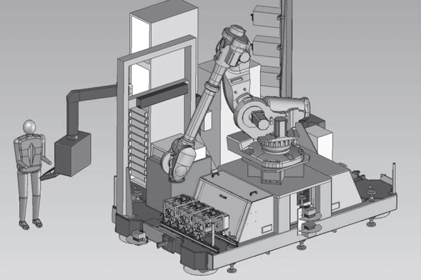
\includegraphics[width=.4\linewidth]{image1}
}%figues de la page de garde

\def\xxtitreexo{Fauteuil dynamique de cinéma}
\def\xxsourceexo{\hspace{.2cm} \footnotesize{Concours Centrale-Supélec TSI 2015}}

\iflivret
\pagestyle{empty}


%%%%%%%% PAGE DE GARDE COURS
\ifcours
\begin{tikzpicture}[remember picture,overlay]
\node at (current page.north west)
{\begin{tikzpicture}[remember picture,overlay]
\node[anchor=north west,inner sep=0pt] at (0,0) {\includegraphics[width=\paperwidth]{\thechapterimage}};
\draw[anchor=west] (-2cm,-8cm) node [line width=2pt,rounded corners=15pt,draw=ocre,fill=white,fill opacity=0.6,inner sep=40pt]{\strut\makebox[22cm]{}};
\draw[anchor=west] (1cm,-8cm) node {\huge\sffamily\bfseries\color{black} %
\begin{minipage}{1cm}
\rotatebox{90}{\LARGE\sffamily\textsc{\color{ocre}\textbf{\xxnumpartie}}}
\end{minipage} \hfill
\begin{minipage}[c]{14cm}
\begin{titrepartie}
\begin{flushright}
\renewcommand{\baselinestretch}{1.1} 
\Large\sffamily\textsc{\textbf{\xxpartie}}
\renewcommand{\baselinestretch}{1} 
\end{flushright}
\end{titrepartie}
\end{minipage} \hfill
\begin{minipage}[c]{3.5cm}
{\large\sffamily\textsc{\textbf{\color{ocre} \discipline}}}
\end{minipage} 
 };
\end{tikzpicture}};
\end{tikzpicture}


\begin{tikzpicture}[overlay]
\node[shape=rectangle, 
      rounded corners = .25 cm,
	  draw= ocre,
	  line width=2pt, 
	  fill = ocre!10,
	  minimum width  = 2.5cm,
	  minimum height = 3cm,] at (18cm,0) {};
\node at (17.7cm,0) {\rotatebox{90}{\textbf{\Large\color{ocre}{\classe}}}};
%{};
\end{tikzpicture}

\vspace{3.5cm}

\begin{tikzpicture}[remember picture,overlay]
\draw[anchor=west] (-2cm,-6cm) node {\huge\sffamily\bfseries\color{black} %
\begin{minipage}{2cm}
\begin{center}
\LARGE\sffamily\textsc{\color{ocre}\textbf{\xxactivite}}
\end{center}
\end{minipage} \hfill
\begin{minipage}[c]{15cm}
\begin{titrechapitre}
\renewcommand{\baselinestretch}{1.1} 
\Large\sffamily\textsc{\textbf{\xxnumchapitre}}

\Large\sffamily\textsc{\textbf{\xxchapitre}}
\vspace{.5cm}

\renewcommand{\baselinestretch}{1} 
\normalsize\normalfont
\xxcompetences
\end{titrechapitre}
\end{minipage}  };
\end{tikzpicture}
\vfill

\begin{flushright}
\begin{minipage}[c]{.3\linewidth}
\begin{center}
\xxfigures
\end{center}
\end{minipage}\hfill
\begin{minipage}[c]{.6\linewidth}
\startcontents
\printcontents{}{1}{}
\end{minipage}
\end{flushright}

\begin{tikzpicture}[remember picture,overlay]
\draw[anchor=west] (4.5cm,-.7cm) node {
\begin{minipage}[c]{.2\linewidth}
\begin{flushright}

\includegraphics[width=2cm]{logoCC}
\end{flushright}
\end{minipage}
\begin{minipage}[c]{.2\linewidth}
\textsl{\xxauteur} \\
\textsl{\classe}
\end{minipage}
 };
\end{tikzpicture}
\newpage
\pagestyle{fancy}

\newpage
\pagestyle{fancy}

\else
\fi


%%%%%%%% PAGE DE GARDE TD
\iftd
%\begin{tikzpicture}[remember picture,overlay]
%\node at (current page.north west)
%{\begin{tikzpicture}[remember picture,overlay]
%\draw[anchor=west] (-2cm,-3.25cm) node [line width=2pt,rounded corners=15pt,draw=ocre,fill=white,fill opacity=0.6,inner sep=40pt]{\strut\makebox[22cm]{}};
%\draw[anchor=west] (1cm,-3.25cm) node {\huge\sffamily\bfseries\color{black} %
%\begin{minipage}{1cm}
%\rotatebox{90}{\LARGE\sffamily\textsc{\color{ocre}\textbf{\xxnumpartie}}}
%\end{minipage} \hfill
%\begin{minipage}[c]{13.5cm}
%\begin{titrepartie}
%\begin{flushright}
%\renewcommand{\baselinestretch}{1.1} 
%\Large\sffamily\textsc{\textbf{\xxpartie}}
%\renewcommand{\baselinestretch}{1} 
%\end{flushright}
%\end{titrepartie}
%\end{minipage} \hfill
%\begin{minipage}[c]{3.5cm}
%{\large\sffamily\textsc{\textbf{\color{ocre} \discipline}}}
%\end{minipage} 
% };
%\end{tikzpicture}};
%\end{tikzpicture}

%%%%%%%%%% PAGE DE GARDE TD %%%%%%%%%%%%%%%
%\begin{tikzpicture}[overlay]
%\node[shape=rectangle, 
%      rounded corners = .25 cm,
%	  draw= ocre,
%	  line width=2pt, 
%	  fill = ocre!10,
%	  minimum width  = 2.5cm,
%	  minimum height = 2.5cm,] at (18.5cm,0) {};
%\node at (17.7cm,0) {\rotatebox{90}{\textbf{\Large\color{ocre}{\classe}}}};
%%{};
%\end{tikzpicture}

% PARTIE ET CHAPITRE
%\begin{tikzpicture}[remember picture,overlay]
%\draw[anchor=west] (-1cm,-2.1cm) node {\large\sffamily\bfseries\color{black} %
%\begin{minipage}[c]{15cm}
%\begin{flushleft}
%\xxnumchapitre \\
%\xxchapitre
%\end{flushleft}
%\end{minipage}  };
%\end{tikzpicture}

% Bandeau titre exo
\begin{tikzpicture}[remember picture,overlay]
\draw[anchor=west] (-2cm,-4cm) node {\huge\sffamily\bfseries\color{black} %
\begin{minipage}{5cm}
\begin{center}
\LARGE\sffamily\color{ocre}\textbf{\textsc{\xxactivite}}

\begin{center}
\xxfigures
\end{center}

\end{center}
\end{minipage} \hfill
\begin{minipage}[c]{12cm}
\begin{titrechapitre}
\renewcommand{\baselinestretch}{1.1} 
\large\sffamily\textbf{\textsc{\xxtitreexo}}

\small\sffamily{\textbf{\textit{\color{black!70}\xxsourceexo}}}
\vspace{.5cm}

\renewcommand{\baselinestretch}{1} 
\normalsize\normalfont
\xxcompetences
\end{titrechapitre}
\end{minipage}  };
\end{tikzpicture}

\else
\fi


%%%%%%%% PAGE DE GARDE FICHE
\iffiche
\begin{tikzpicture}[remember picture,overlay]
\node at (current page.north west)
{\begin{tikzpicture}[remember picture,overlay]
\draw[anchor=west] (-2cm,-3.25cm) node [line width=2pt,rounded corners=15pt,draw=ocre,fill=white,fill opacity=0.6,inner sep=40pt]{\strut\makebox[22cm]{}};
\draw[anchor=west] (1cm,-3.25cm) node {\huge\sffamily\bfseries\color{black} %
\begin{minipage}{1cm}
\rotatebox{90}{\LARGE\sffamily\textsc{\color{ocre}\textbf{\xxnumpartie}}}
\end{minipage} \hfill
\begin{minipage}[c]{14cm}
\begin{titrepartie}
\begin{flushright}
\renewcommand{\baselinestretch}{1.1} 
\large\sffamily\textsc{\textbf{\xxpartie} \\} 

\vspace{.2cm}

\normalsize\sffamily\textsc{\textbf{\xxnumchapitre -- \xxchapitre}}
\renewcommand{\baselinestretch}{1} 
\end{flushright}
\end{titrepartie}
\end{minipage} \hfill
\begin{minipage}[c]{3.5cm}
{\large\sffamily\textsc{\textbf{\color{ocre} \discipline}}}
\end{minipage} 
 };
\end{tikzpicture}};
\end{tikzpicture}


\begin{tikzpicture}[overlay]
\node[shape=rectangle, 
      rounded corners = .25 cm,
	  draw= ocre,
	  line width=2pt, 
	  fill = ocre!10,
	  minimum width  = 2.5cm,
	  minimum height = 2.5cm,] at (18.5cm,0.5cm) {};
%	  minimum height = 2.5cm,] at (18.5cm,0cm) {};
\node at (17.7cm,0.5) {\rotatebox{90}{\textsf{\textbf{\large\color{ocre}{\classe}}}}};
%{};
\end{tikzpicture}



\else
\fi



\else
\pagestyle{empty}


%%%%%%%% PAGE DE GARDE COURS
\ifcours
\begin{tikzpicture}[remember picture,overlay]
\node at (current page.north west)
{\begin{tikzpicture}[remember picture,overlay]
\node[anchor=north west,inner sep=0pt] at (0,0) {\includegraphics[width=\paperwidth]{\thechapterimage}};
\draw[anchor=west] (-2cm,-8cm) node [line width=2pt,rounded corners=15pt,draw=ocre,fill=white,fill opacity=0.6,inner sep=40pt]{\strut\makebox[22cm]{}};
\draw[anchor=west] (1cm,-8cm) node {\huge\sffamily\bfseries\color{black} %
\begin{minipage}{1cm}
\rotatebox{90}{\LARGE\sffamily\textsc{\color{ocre}\textbf{\xxnumpartie}}}
\end{minipage} \hfill
\begin{minipage}[c]{14cm}
\begin{titrepartie}
\begin{flushright}
\renewcommand{\baselinestretch}{1.1} 
\Large\sffamily\textsc{\textbf{\xxpartie}}
\renewcommand{\baselinestretch}{1} 
\end{flushright}
\end{titrepartie}
\end{minipage} \hfill
\begin{minipage}[c]{3.5cm}
{\large\sffamily\textsc{\textbf{\color{ocre} \discipline}}}
\end{minipage} 
 };
\end{tikzpicture}};
\end{tikzpicture}


\begin{tikzpicture}[overlay]
\node[shape=rectangle, 
      rounded corners = .25 cm,
	  draw= ocre,
	  line width=2pt, 
	  fill = ocre!10,
	  minimum width  = 2.5cm,
	  minimum height = 3cm,] at (18cm,0) {};
\node at (17.7cm,0) {\rotatebox{90}{\textbf{\Large\color{ocre}{\classe}}}};
%{};
\end{tikzpicture}

\vspace{3.5cm}

\begin{tikzpicture}[remember picture,overlay]
\draw[anchor=west] (-2cm,-6cm) node {\huge\sffamily\bfseries\color{black} %
\begin{minipage}{2cm}
\begin{center}
\LARGE\sffamily\textsc{\color{ocre}\textbf{\xxactivite}}
\end{center}
\end{minipage} \hfill
\begin{minipage}[c]{15cm}
\begin{titrechapitre}
\renewcommand{\baselinestretch}{1.1} 
\Large\sffamily\textsc{\textbf{\xxnumchapitre}}

\Large\sffamily\textsc{\textbf{\xxchapitre}}
\vspace{.5cm}

\renewcommand{\baselinestretch}{1} 
\normalsize\normalfont
\xxcompetences
\end{titrechapitre}
\end{minipage}  };
\end{tikzpicture}
\vfill

\begin{flushright}
\begin{minipage}[c]{.3\linewidth}
\begin{center}
\xxfigures
\end{center}
\end{minipage}\hfill
\begin{minipage}[c]{.6\linewidth}
\startcontents
\printcontents{}{1}{}
\end{minipage}
\end{flushright}

\begin{tikzpicture}[remember picture,overlay]
\draw[anchor=west] (4.5cm,-.7cm) node {
\begin{minipage}[c]{.2\linewidth}
\begin{flushright}

\includegraphics[width=2cm]{logoCC}
\end{flushright}
\end{minipage}
\begin{minipage}[c]{.2\linewidth}
\textsl{\xxauteur} \\
\textsl{\classe}
\end{minipage}
 };
\end{tikzpicture}
\newpage
\pagestyle{fancy}

\newpage
\pagestyle{fancy}

\else
\fi


%%%%%%%% PAGE DE GARDE TD
\iftd
%\begin{tikzpicture}[remember picture,overlay]
%\node at (current page.north west)
%{\begin{tikzpicture}[remember picture,overlay]
%\draw[anchor=west] (-2cm,-3.25cm) node [line width=2pt,rounded corners=15pt,draw=ocre,fill=white,fill opacity=0.6,inner sep=40pt]{\strut\makebox[22cm]{}};
%\draw[anchor=west] (1cm,-3.25cm) node {\huge\sffamily\bfseries\color{black} %
%\begin{minipage}{1cm}
%\rotatebox{90}{\LARGE\sffamily\textsc{\color{ocre}\textbf{\xxnumpartie}}}
%\end{minipage} \hfill
%\begin{minipage}[c]{13.5cm}
%\begin{titrepartie}
%\begin{flushright}
%\renewcommand{\baselinestretch}{1.1} 
%\Large\sffamily\textsc{\textbf{\xxpartie}}
%\renewcommand{\baselinestretch}{1} 
%\end{flushright}
%\end{titrepartie}
%\end{minipage} \hfill
%\begin{minipage}[c]{3.5cm}
%{\large\sffamily\textsc{\textbf{\color{ocre} \discipline}}}
%\end{minipage} 
% };
%\end{tikzpicture}};
%\end{tikzpicture}

%%%%%%%%%% PAGE DE GARDE TD %%%%%%%%%%%%%%%
%\begin{tikzpicture}[overlay]
%\node[shape=rectangle, 
%      rounded corners = .25 cm,
%	  draw= ocre,
%	  line width=2pt, 
%	  fill = ocre!10,
%	  minimum width  = 2.5cm,
%	  minimum height = 2.5cm,] at (18.5cm,0) {};
%\node at (17.7cm,0) {\rotatebox{90}{\textbf{\Large\color{ocre}{\classe}}}};
%%{};
%\end{tikzpicture}

% PARTIE ET CHAPITRE
%\begin{tikzpicture}[remember picture,overlay]
%\draw[anchor=west] (-1cm,-2.1cm) node {\large\sffamily\bfseries\color{black} %
%\begin{minipage}[c]{15cm}
%\begin{flushleft}
%\xxnumchapitre \\
%\xxchapitre
%\end{flushleft}
%\end{minipage}  };
%\end{tikzpicture}

% Bandeau titre exo
\begin{tikzpicture}[remember picture,overlay]
\draw[anchor=west] (-2cm,-4cm) node {\huge\sffamily\bfseries\color{black} %
\begin{minipage}{5cm}
\begin{center}
\LARGE\sffamily\color{ocre}\textbf{\textsc{\xxactivite}}

\begin{center}
\xxfigures
\end{center}

\end{center}
\end{minipage} \hfill
\begin{minipage}[c]{12cm}
\begin{titrechapitre}
\renewcommand{\baselinestretch}{1.1} 
\large\sffamily\textbf{\textsc{\xxtitreexo}}

\small\sffamily{\textbf{\textit{\color{black!70}\xxsourceexo}}}
\vspace{.5cm}

\renewcommand{\baselinestretch}{1} 
\normalsize\normalfont
\xxcompetences
\end{titrechapitre}
\end{minipage}  };
\end{tikzpicture}

\else
\fi


%%%%%%%% PAGE DE GARDE FICHE
\iffiche
\begin{tikzpicture}[remember picture,overlay]
\node at (current page.north west)
{\begin{tikzpicture}[remember picture,overlay]
\draw[anchor=west] (-2cm,-3.25cm) node [line width=2pt,rounded corners=15pt,draw=ocre,fill=white,fill opacity=0.6,inner sep=40pt]{\strut\makebox[22cm]{}};
\draw[anchor=west] (1cm,-3.25cm) node {\huge\sffamily\bfseries\color{black} %
\begin{minipage}{1cm}
\rotatebox{90}{\LARGE\sffamily\textsc{\color{ocre}\textbf{\xxnumpartie}}}
\end{minipage} \hfill
\begin{minipage}[c]{14cm}
\begin{titrepartie}
\begin{flushright}
\renewcommand{\baselinestretch}{1.1} 
\large\sffamily\textsc{\textbf{\xxpartie} \\} 

\vspace{.2cm}

\normalsize\sffamily\textsc{\textbf{\xxnumchapitre -- \xxchapitre}}
\renewcommand{\baselinestretch}{1} 
\end{flushright}
\end{titrepartie}
\end{minipage} \hfill
\begin{minipage}[c]{3.5cm}
{\large\sffamily\textsc{\textbf{\color{ocre} \discipline}}}
\end{minipage} 
 };
\end{tikzpicture}};
\end{tikzpicture}


\begin{tikzpicture}[overlay]
\node[shape=rectangle, 
      rounded corners = .25 cm,
	  draw= ocre,
	  line width=2pt, 
	  fill = ocre!10,
	  minimum width  = 2.5cm,
	  minimum height = 2.5cm,] at (18.5cm,0.5cm) {};
%	  minimum height = 2.5cm,] at (18.5cm,0cm) {};
\node at (17.7cm,0.5) {\rotatebox{90}{\textsf{\textbf{\large\color{ocre}{\classe}}}}};
%{};
\end{tikzpicture}



\else
\fi



\fi
\setlength{\columnseprule}{.1pt}

\pagestyle{fancy}
\thispagestyle{plain}


\vspace{4.5cm}

\def\columnseprulecolor{\color{ocre}}
\setlength{\columnseprule}{0.4pt} 

%%%%%%%%%%%%%%
%\documentclass[10pt,fleqn]{article} % Default font size and left-justified equations
%\usepackage[%
%    pdftitle={Modélisation SLCI : Rapidité des systèmes},
%    pdfauthor={Xavier Pessoles}]{hyperref}
%    
%%%%%%%%%%%%%%%%%%%%%%%%%%%%%%%%%%%%%%%%%%
% Original author:
% Mathias Legrand (legrand.mathias@gmail.com) with modifications by:
% Vel (vel@latextemplates.com)
% License:
% CC BY-NC-SA 3.0 (http://creativecommons.org/licenses/by-nc-sa/3.0/)
%%%%%%%%%%%%%%%%%%%%%%%%%%%%%%%%%%%%%%%%%

%----------------------------------------------------------------------------------------
%	VARIOUS REQUIRED PACKAGES AND CONFIGURATIONS
%----------------------------------------------------------------------------------------

%\usepackage[top=2.5cm,bottom=2cm,left=2cm,right=2cm,headsep=40pt,a4paper]{geometry} % Page margins
\usepackage[top=2cm,bottom=3cm,left=2cm,right=2cm,a4paper]{geometry} % Page margins

\usepackage{graphicx} % Required for including pictures

\usepackage{lipsum} % Inserts dummy text

\usepackage{tikz} % Required for drawing custom shapes

\usepackage[francais]{babel} % English language/hyphenation
\frenchbsetup{StandardLists=true} % Pour éviter la collision babel enumitem pour les listes

\usepackage{enumitem} % Customize lists
\setlist{nolistsep} % Reduce spacing between bullet points and numbered lists

\usepackage{booktabs} % Required for nicer horizontal rules in tables

\usepackage{xcolor} % Required for specifying colors by name
%\definecolor{ocre}{RGB}{243,102,25} % Define the orange color used for highlighting throughout the book
 \definecolor{ocre}{RGB}{49,133,156} % Couleur ''bleue''
\definecolor{violetf}{RGB}{112,48,160} % Couleur ''violet''
\usepackage{enumitem}
\usepackage{pifont} % Pour les dinglist
\usepackage{multicol}
\usepackage{array} % Centrage vertical dans les tableaux

%----------------------------------------------------------------------------------------
%	FONTS
%----------------------------------------------------------------------------------------

\usepackage{multicol}
\usepackage{siunitx}
\sisetup{output-decimal-marker = {,}}


\usepackage{avant} % Use the Avantgarde font for headings
%\usepackage{times} % Use the Times font for headings
%\usepackage{mathptmx} % Use the Adobe Times Roman as the default text font together with math symbols from the Sym­bol, Chancery and Com­puter Modern fonts
\usepackage[adobe-utopia]{mathdesign}
\usepackage{microtype} % Slightly tweak font spacing for aesthetics
\usepackage[utf8]{inputenc} % Required for including letters with accents
\usepackage[T1]{fontenc} % Use 8-bit encoding that has 256 glyphs

%----------------------------------------------------------------------------------------
%	BIBLIOGRAPHY AND INDEX
%----------------------------------------------------------------------------------------

%\usepackage[style=alphabetic,citestyle=numeric,sorting=nyt,sortcites=true,autopunct=true,babel=hyphen,hyperref=true,abbreviate=false,backref=true,backend=biber]{biblatex}
\usepackage[style=alphabetic,citestyle=numeric,sorting=nyt,sortcites=true,autopunct=true,hyperref=true,abbreviate=false,backref=true,backend=biber]{biblatex}
\addbibresource{bibliography.bib} % BibTeX bibliography file
\defbibheading{bibempty}{}

\usepackage{calc} % For simpler calculation - used for spacing the index letter headings correctly
\usepackage{makeidx} % Required to make an index
\makeindex % Tells LaTeX to create the files required for indexing

%----------------------------------------------------------------------------------------
%	MAIN TABLE OF CONTENTS
%----------------------------------------------------------------------------------------

\usepackage{titletoc} % Required for manipulating the table of contents

\setcounter{tocdepth}{2}     % Dans la table des matieres
\setcounter{secnumdepth}{2}

\contentsmargin{0cm} % Removes the default margin

% Part text styling
\titlecontents{part}[0cm]
{\addvspace{20pt}\centering\large\bfseries}
{}
{}
{}

% Chapter text styling
\titlecontents{chapter}[1.25cm] % Indentation
{\addvspace{12pt}\large\sffamily\bfseries} % Spacing and font options for chapters
{\color{ocre!60}\contentslabel[\Large\thecontentslabel]{1.25cm}\color{ocre}} % Chapter number
{\color{ocre}}  
{\color{ocre!60}\normalsize\;\titlerule*[.5pc]{.}\;\thecontentspage} % Page number

% Section text styling
\titlecontents{section}[1.25cm] % Indentation
{\addvspace{3pt}\sffamily\bfseries} % Spacing and font options for sections
{\color{ocre!60}\contentslabel[\thecontentslabel]{1.25cm} \color{ocre}} % Section number
{\color{ocre}}
{\hfill\color{ocre!60}\thecontentspage} % Page number
[]

% Subsection text styling
\titlecontents{subsection}[1.25cm] % Indentation
{\addvspace{1pt}\sffamily\small} % Spacing and font options for subsections
{\contentslabel[\thecontentslabel]{1.25cm}} % Subsection number
{}
{\ \titlerule*[.5pc]{.}\;\thecontentspage} % Page number
[]


% Subsection text styling
\titlecontents{subsubsection}[1.25cm] % Indentation
{\addvspace{1pt}\sffamily\small} % Spacing and font options for subsections
{\contentslabel[\thecontentslabel]{1.25cm}} % Subsection number
{}
{\ \titlerule*[.5pc]{.}\;\thecontentspage} % Page number
[]

% List of figures
\titlecontents{figure}[0em]
{\addvspace{-5pt}\sffamily}
{\thecontentslabel\hspace*{1em}}
{}
{\ \titlerule*[.5pc]{.}\;\thecontentspage}
[]

% List of tables
\titlecontents{table}[0em]
{\addvspace{-5pt}\sffamily}
{\thecontentslabel\hspace*{1em}}
{}
{\ \titlerule*[.5pc]{.}\;\thecontentspage}
[]

%----------------------------------------------------------------------------------------
%	MINI TABLE OF CONTENTS IN PART HEADS
%----------------------------------------------------------------------------------------

% Chapter text styling
\titlecontents{lchapter}[0em] % Indenting
{\addvspace{15pt}\large\sffamily\bfseries} % Spacing and font options for chapters
{\color{ocre}\contentslabel[\Large\thecontentslabel]{1.25cm}\color{ocre}} % Chapter number
{}  
{\color{ocre}\normalsize\sffamily\bfseries\;\titlerule*[.5pc]{.}\;\thecontentspage} % Page number

% Section text styling
\titlecontents{lsection}[0em] % Indenting
{\sffamily\small} % Spacing and font options for sections
{\contentslabel[\thecontentslabel]{1.25cm}} % Section number
{}
{}

% Subsection text styling
\titlecontents{lsubsection}[.5em] % Indentation
{\normalfont\footnotesize\sffamily} % Font settings
{}
{}
{}

%----------------------------------------------------------------------------------------
%	PAGE HEADERS
%----------------------------------------------------------------------------------------

\usepackage{fancyhdr} % Required for header and footer configuration



\pagestyle{fancy}
 \renewcommand{\headrulewidth}{0pt}
 \fancyhead{}
 
 % ENTETES de page
 \fancyhead[L]{%
 \noindent\begin{minipage}[c]{2.6cm}%
 
\includegraphics[width=2cm]{logo_lycee.png}%
 \end{minipage}}

\fancyhead[C]{\rule{8cm}{.5pt}}

 \fancyhead[R]{%
 \noindent\begin{minipage}[c]{3cm}
 \begin{flushright}
 \footnotesize{\textit{\textsf{\xxtete}}}%
 \end{flushright}
 \end{minipage}
}

 \fancyfoot{}
 % PIEDS de page
\fancyfoot[C]{\rule{12cm}{.5pt}}
\renewcommand{\footrulewidth}{0.2pt}
\fancyfoot[C]{\footnotesize{\bfseries \thepage}}
\fancyfoot[L]{ 
\begin{minipage}[c]{.4\linewidth}
\noindent\footnotesize{{\xxauteur}}
\end{minipage}}

\fancyfoot[R]{\footnotesize{\xxpied}
\ifthenelse{\isodd{\value{page}}}{
\begin{tikzpicture}[overlay]
\node[shape=rectangle, 
      rounded corners = .25 cm,
	  draw= ocre,
	  line width=2pt, 
	  fill = ocre!10,
	  minimum width  = 2.5cm,
	  minimum height = 3cm,] at (\xxposongletx,\xxposonglety) {};
\node at (\xxposonglettext,\xxposonglety) {\rotatebox{90}{\textbf{\large\color{ocre}{\xxonglet}}}};
%{};
\end{tikzpicture}}{}
}



%
%
%
% Removes the header from odd empty pages at the end of chapters
\makeatletter
%\renewcommand{\cleardoublepage}{
%\clearpage\ifodd\c@page\else
%\hbox{}
%\vspace*{\fill}
%\thispagestyle{empty}
%\newpage
%\fi}

%\fancypagestyle{plain}{%
%\fancyhf{} % vide l’en-tête et le pied~de~page.
%%\fancyfoot[C]{\bfseries \thepage} % numéro de la page en cours en gras
%% et centré en pied~de~page.
%\fancyfoot[R]{\footnotesize{\xxpied}}
%\fancyfoot[C]{\rule{12cm}{.5pt}}
%\renewcommand{\footrulewidth}{0.2pt}
%\fancyfoot[C]{\footnotesize{\bfseries \thepage}}
%\fancyfoot[L]{ 
%\begin{minipage}[c]{.4\linewidth}
%\noindent\footnotesize{{\xxauteur}}
%\end{minipage}}}

\fancypagestyle{plain}{%
\fancyhf{} % vide l’en-tête et le pied~de~page.
\fancyfoot[C]{\rule{12cm}{.5pt}}
\renewcommand{\footrulewidth}{0.2pt}
\fancyfoot[C]{\footnotesize{\bfseries \thepage}}
\fancyfoot[L]{ 
\begin{minipage}[c]{.4\linewidth}
\noindent\footnotesize{{\xxauteur}}
\end{minipage}}
\fancyfoot[R]{\footnotesize{\xxpied}}
}



%----------------------------------------------------------------------------------------
%	THEOREM STYLES
%----------------------------------------------------------------------------------------

% Conflit avec la police adobe
%\usepackage{amsmath,amsfonts,amssymb,amsthm} % For math equations, theorems, symbols, etc
\usepackage{amsmath,amsthm}

\newcommand{\intoo}[2]{\mathopen{]}#1\,;#2\mathclose{[}}
\newcommand{\ud}{\mathop{\mathrm{{}d}}\mathopen{}}
\newcommand{\intff}[2]{\mathopen{[}#1\,;#2\mathclose{]}}
%\newtheorem{notation}{Notation}[chapter]
\newtheorem{notation}{Notation}[section]

% Boxed/framed environments
\newtheoremstyle{ocrenumbox}% % Theorem style name
{0pt}% Space above
{0pt}% Space below
{\normalfont}% % Body font
{}% Indent amount
{\small\bf\sffamily\color{ocre}}% % Theorem head font
{\;}% Punctuation after theorem head
{0.25em}% Space after theorem head
{\small\sffamily\color{ocre}\thmname{#1}\nobreakspace\thmnumber%{\@ifnotempty{#1}{}\@upn{#2}}% Theorem text (e.g. Theorem 2.1)
\thmnote{\nobreakspace\the\thm@notefont\sffamily\bfseries\color{black}---\nobreakspace#3.}} % Optional theorem note
\renewcommand{\qedsymbol}{$\blacksquare$}% Optional qed square


% Boite pour les corriges
\newtheoremstyle{correctionbox}% % Theorem style name
{0pt}% Space above
{0pt}% Space below
{\normalfont}% % Body font
{}% Indent amount
{\small\bf\sffamily\color{violet}}% % Theorem head font
{\;}% Punctuation after theorem head
{0.25em}% Space after theorem head
{\small\sffamily\color{ocre}\thmname{#1}\nobreakspace\thmnumber%{\@ifnotempty{#1}{}\@upn{#2}}% Theorem text (e.g. Theorem 2.1)
\thmnote{\nobreakspace\the\thm@notefont\sffamily\bfseries\color{black}---\nobreakspace#3.}} % Optional theorem note
\renewcommand{\qedsymbol}{$\blacksquare$}% Optional qed square



\newtheoremstyle{blacknumex}% Theorem style name
{5pt}% Space above
{5pt}% Space below
{\normalfont}% Body font
{} % Indent amount
{\small\bf\sffamily}% Theorem head font
{\;}% Punctuation after theorem head
{0.25em}% Space after theorem head
{\small\sffamily{\tiny\ensuremath{\blacksquare}}\nobreakspace\thmname{#1}\nobreakspace\thmnumber%{\@ifnotempty{#1}{}\@upn{#2}}% Theorem text (e.g. Theorem 2.1)
\thmnote{\nobreakspace\the\thm@notefont\sffamily\bfseries---\nobreakspace#3.}}% Optional theorem note

\newtheoremstyle{blacknumbox} % Theorem style name
{0pt}% Space above
{0pt}% Space below
{\normalfont}% Body font
{}% Indent amount
{\small\bf\sffamily}% Theorem head font
{\;}% Punctuation after theorem head
{0.25em}% Space after theorem head
{\small\sffamily\thmname{#1}\nobreakspace 
\thmnote{\nobreakspace\the\thm@notefont\sffamily\bfseries---\nobreakspace#3.}}% Optional theorem note

% Non-boxed/non-framed environments
\newtheoremstyle{ocrenum}% % Theorem style name
{5pt}% Space above
{5pt}% Space below
{\normalfont}% % Body font
{}% Indent amount
{\small\bf\sffamily\color{ocre}}% % Theorem head font
{\;}% Punctuation after theorem head
{0.25em}% Space after theorem head
{\small\sffamily\color{ocre}\thmname{#1}\nobreakspace%\thmnumber{\@ifnotempty{#1}{}\@upn{#2}}% Theorem text (e.g. Theorem 2.1)
\thmnote{\nobreakspace\the\thm@notefont\sffamily\bfseries\color{black}---\nobreakspace#3.}} % Optional theorem note
\renewcommand{\qedsymbol}{$\blacksquare$}% Optional qed square
\makeatother

% Environnement pour les titres de parties
\newtheoremstyle{partiebox} 
{0pt}% Space above
{0pt}% Space below
{\normalfont}% Body font
{}% Indent amount
{\small\bf\sffamily}% Theorem head font
{\;}% Punctuation after theorem head
{0.25em}% Space after theorem head




% Defines the theorem text style for each type of theorem to one of the three styles above
\newcounter{dummy} 
\numberwithin{dummy}{section}
\theoremstyle{ocrenumbox}
%\newtheorem{theoremeT}[dummy]{Théorème}
\newtheorem{theoremeT}[dummy]{Théorème}
\newtheorem{resultatT}[dummy]{Résultat}
\newtheorem{savoirT}[dummy]{Savoir}
\newtheorem{methodeT}[dummy]{Méthode}
\newtheorem{objectifT}[dummy]{Objectif}
%\newtheorem{problem}{Problem}[chapter]
\newtheorem{problem}{Problem}[section]
%\newtheorem{exerciseT}{Exercise}[chapter]
\newtheorem{exerciseT}{Exercice}[section]

\theoremstyle{blacknumex}
%\newtheorem{exampleT}{Example}[chapter]
\newtheorem{exempleT}{Exemple}[section]
\newtheorem{termT}{Terminal\\}[section]
\newtheorem{pyT}{Python\\}[section]
\newtheorem{sciT}{Scilab\\}[section]
\newtheorem{pseudoT}{Pseudo Code\\}[section]
\newtheorem{sqlT}{SQL\\}[section]

\theoremstyle{blacknumbox}
%\newtheorem{vocabulary}{Vocabulary}[chapter]
\newtheorem{vocabulary}{Vocabulaire}[section]
%\newtheorem{definitionT}{Definition}[section]
\newtheorem{definitionT}{Définition}[section]
\newtheorem{rappelT}{Rappel}[section]
\newtheorem{demoT}{Démonstration}[section]
\newtheorem{corollaryT}[dummy]{Corollaire}
\newtheorem{hypoT}{Hypothèse(s)}

\theoremstyle{ocrenum}
\newtheorem{proposition}[dummy]{Proposition}

\theoremstyle{partiebox}
\newtheorem{titrepartieT}[]{}
\newtheorem{titrechapitreT}[]{}

\theoremstyle{correctionbox}
\newtheorem{correctionT}[dummy]{\color{violet}{Correction}}

%----------------------------------------------------------------------------------------
%	DEFINITION OF COLORED BOXES
%----------------------------------------------------------------------------------------

\RequirePackage[framemethod=tikz]{mdframed} % Required for creating the theorem, definition, exercise and corollary boxes

% Theorem box
\newmdenv[skipabove=7pt,
skipbelow=7pt,
backgroundcolor=ocre!10,
linecolor=ocre,
innerleftmargin=5pt,
innerrightmargin=5pt,
innertopmargin=5pt,
leftmargin=0cm,
rightmargin=0cm,
innerbottommargin=5pt]{tBox}


% Correction
\newmdenv[skipabove=7pt,
skipbelow=7pt,
backgroundcolor=violet!10,
linecolor=violet,
innerleftmargin=5pt,
innerrightmargin=5pt,
innertopmargin=5pt,
leftmargin=0cm,
rightmargin=0cm,
innerbottommargin=5pt]{coBox}


% Exercise box	  
\newmdenv[skipabove=7pt,
skipbelow=7pt,
rightline=false,
leftline=true,
topline=false,
bottomline=false,
backgroundcolor=ocre!10,
linecolor=ocre,
innerleftmargin=5pt,
innerrightmargin=5pt,
innertopmargin=5pt,
innerbottommargin=5pt,
leftmargin=0cm,
rightmargin=0cm,
linewidth=4pt]{eBox}	

% Definition box
\newmdenv[skipabove=7pt,
skipbelow=7pt,
rightline=false,
leftline=true,
topline=false,
bottomline=false,
backgroundcolor=ocre!10,
linecolor=ocre,
innerleftmargin=5pt,
innerrightmargin=5pt,
innertopmargin=0pt,
leftmargin=0cm,
rightmargin=0cm,
linewidth=4pt,
innerbottommargin=0pt]{dBox}	

% Demonstration box
\newmdenv[skipabove=7pt,
skipbelow=7pt,
rightline=false,
leftline=true,
topline=false,
bottomline=false,
%backgroundcolor=ocre!10,
linecolor=ocre,
innerleftmargin=5pt,
innerrightmargin=5pt,
innertopmargin=0pt,
leftmargin=0cm,
rightmargin=0cm,
linewidth=4pt,
innerbottommargin=0pt]{demoBox}	

% Corollary box
\newmdenv[skipabove=7pt,
skipbelow=7pt,
rightline=false,
leftline=true,
topline=false,
bottomline=false,
linecolor=gray,
backgroundcolor=black!5,
innerleftmargin=5pt,
innerrightmargin=5pt,
innertopmargin=5pt,
leftmargin=0cm,
rightmargin=0cm,
linewidth=4pt,
innerbottommargin=5pt]{cBox}


% Hypothèses
\newmdenv[skipabove=7pt,
skipbelow=7pt,
rightline=false,
leftline=true,
topline=false,
bottomline=false,
linecolor=gray,
backgroundcolor=black!5,
innerleftmargin=5pt,
innerrightmargin=5pt,
innertopmargin=5pt,
leftmargin=0cm,
rightmargin=0cm,
linewidth=4pt,
innerbottommargin=5pt]{hyBox}


% Boite pour le titre de la partie (pBox)
\newmdenv[skipabove=7pt,
skipbelow=7pt,
rightline=true,
leftline=false,
topline=false,
bottomline=false,
linecolor=ocre,
backgroundcolor=none,
innerleftmargin=5pt,
innerrightmargin=5pt,
innertopmargin=5pt,
leftmargin=0cm,
rightmargin=0cm,
linewidth=4pt,
innerbottommargin=5pt]{pBox}

% Boite pour le titre du chapitre (chBox)
\newmdenv[skipabove=7pt,
skipbelow=7pt,
rightline=false,
leftline=true,
topline=false,
bottomline=false,
linecolor=ocre,
%backgroundcolor=black!5,
innerleftmargin=5pt,
innerrightmargin=5pt,
innertopmargin=5pt,
leftmargin=0cm,
rightmargin=0cm,
linewidth=4pt,
innerbottommargin=5pt]{chBox}


% Boite pour les exemples
\newmdenv[skipabove=7pt,
skipbelow=7pt,
rightline=false,
leftline=true,
topline=false,
bottomline=false,
linecolor=gray,
backgroundcolor=white,
innerleftmargin=5pt,
innerrightmargin=5pt,
innertopmargin=5pt,
leftmargin=0cm,
rightmargin=0cm,
linewidth=4pt,
innerbottommargin=5pt]{exBox}

% Boite pour le terminal
\newmdenv[skipabove=7pt,
skipbelow=7pt,
rightline=false,
leftline=true,
topline=false,
bottomline=false,
linecolor=gray,
backgroundcolor=white,
innerleftmargin=5pt,
innerrightmargin=5pt,
innertopmargin=5pt,
leftmargin=0cm,
rightmargin=0cm,
linewidth=4pt,
innerbottommargin=5pt]{termBox}


% Boite pour Python
\newmdenv[skipabove=7pt,
skipbelow=7pt,
rightline=false,
leftline=true,
topline=false,
bottomline=false,
linecolor=gray,
backgroundcolor=white,
innerleftmargin=5pt,
innerrightmargin=5pt,
innertopmargin=0pt,
leftmargin=0cm,
rightmargin=0cm,
linewidth=4pt,
innerbottommargin=5pt]{pyBox}

% Boite pour scilab
\newmdenv[skipabove=7pt,
skipbelow=7pt,
rightline=false,
leftline=true,
topline=false,
bottomline=false,
linecolor=gray,
backgroundcolor=white,
innerleftmargin=5pt,
innerrightmargin=5pt,
innertopmargin=5pt,
leftmargin=0cm,
rightmargin=0cm,
linewidth=4pt,
innerbottommargin=5pt]{sciBox}


% Boite pour pseudo
\newmdenv[skipabove=7pt,
skipbelow=7pt,
rightline=false,
leftline=true,
topline=false,
bottomline=false,
linecolor=gray,
backgroundcolor=white,
innerleftmargin=5pt,
innerrightmargin=5pt,
innertopmargin=5pt,
leftmargin=0cm,
rightmargin=0cm,
linewidth=4pt,
innerbottommargin=5pt]{pseudoBox}

% Boite pour pseudo
\newmdenv[skipabove=7pt,
skipbelow=7pt,
rightline=false,
leftline=true,
topline=false,
bottomline=false,
linecolor=gray,
backgroundcolor=white,
innerleftmargin=5pt,
innerrightmargin=5pt,
innertopmargin=5pt,
leftmargin=0cm,
rightmargin=0cm,
linewidth=4pt,
innerbottommargin=5pt]{sqlBox}


% Creates an environment for each type of theorem and assigns it a theorem text style from the "Theorem Styles" section above and a colored box from above
\newenvironment{theorem}{\begin{tBox}\begin{theoremeT}}{\end{theoremeT}\end{tBox}}
\newenvironment{resultat}{\begin{tBox}\begin{resultatT}}{\end{resultatT}\end{tBox}}
\newenvironment{methode}{\begin{tBox}\begin{methodeT}}{\end{methodeT}\end{tBox}}
\newenvironment{savoir}{\begin{tBox}\begin{savoirT}}{\end{savoirT}\end{tBox}}
\newenvironment{obj}{\begin{tBox}\begin{objectifT}}{\end{objectifT}\end{tBox}}
\newenvironment{corrige}{\begin{coBox}\begin{correctionT}}{\end{correctionT}\end{coBox}}
\newenvironment{exercise}{\begin{eBox}\begin{exerciseT}}{\hfill{\color{ocre}\tiny\ensuremath{\blacksquare}}\end{exerciseT}\end{eBox}}				  
\newenvironment{exercice}{\begin{eBox}\begin{exerciseT}}{\hfill{\color{ocre}\tiny\ensuremath{\blacksquare}}\end{exerciseT}\end{eBox}}				  

\newenvironment{definition}{\begin{dBox}\begin{definitionT}}{\end{definitionT}\end{dBox}}	
\newenvironment{rappel}{\begin{dBox}\begin{rappelT}}{\end{rappelT}\end{dBox}}	
\newenvironment{defi}{\begin{dBox}\begin{definitionT}}{\end{definitionT}\end{dBox}}	
\newenvironment{demo}{\begin{demoBox}\begin{demoT}}{\end{demoT}\end{demoBox}}	
%\newenvironment{exemple}{\begin{exempleT}}{\hfill{\tiny\ensuremath{\blacksquare}}\end{exempleT}}		
\newenvironment{corollary}{\begin{cBox}\begin{corollaryT}}{\end{corollaryT}\end{cBox}}
\newenvironment{hypo}{\begin{hyBox}\begin{hypoT}}{\end{hypoT}\end{hyBox}}	\newenvironment{exemple}{\begin{exBox}\begin{exempleT}}{\hfill{\tiny\ensuremath{\blacksquare}}\end{exempleT}\end{exBox}}	
\newenvironment{titrepartie}{\begin{pBox}\begin{titrepartieT}}{\end{titrepartieT}\end{pBox}}	
\newenvironment{titrechapitre}{\begin{chBox}\begin{titrechapitreT}}{\end{titrechapitreT}\end{chBox}}	

\newenvironment{term}{ \begin{termBox}\begin{termT}}{\end{termT}\end{termBox}}
\newenvironment{py}{ \begin{pyBox}\begin{pyT}}{\end{pyT}\end{pyBox}}
\newenvironment{sci}{ \begin{sciBox}\begin{sciT}}{\end{sciT}\end{sciBox}}
\newenvironment{pseudo}{ \begin{pseudoBox}\begin{pseudoT}}{\end{pseudoT}\end{pseudoBox}}
\newenvironment{envsql}{ \begin{sqlBox}\begin{sqlT}}{\end{sqlT}\end{sqlBox}}


%----------------------------------------------------------------------------------------
%	REMARK ENVIRONMENT
%----------------------------------------------------------------------------------------

\newenvironment{remark}{\par\vspace{10pt}\small % Vertical white space above the remark and smaller font size
\begin{list}{}{
\leftmargin=35pt % Indentation on the left
\rightmargin=25pt}\item\ignorespaces % Indentation on the right
\makebox[-2.5pt]{\begin{tikzpicture}[overlay]
\node[draw=ocre!60,line width=1pt,circle,fill=ocre!25,font=\sffamily\bfseries,inner sep=2pt,outer sep=0pt] at (-15pt,0pt){\textcolor{ocre}{R}};\end{tikzpicture}} % Orange R in a circle
\advance\baselineskip -1pt}{\end{list}\vskip5pt} % Tighter line spacing and white space after remark

\newenvironment{rem}{\par\vspace{10pt}\small % Vertical white space above the remark and smaller font size
\begin{list}{}{
\leftmargin=35pt % Indentation on the left
\rightmargin=25pt}\item\ignorespaces % Indentation on the right
\makebox[-2.5pt]{\begin{tikzpicture}[overlay]
\node[draw=ocre!60,line width=1pt,circle,fill=ocre!25,font=\sffamily\bfseries,inner sep=2pt,outer sep=0pt] at (-15pt,0pt){\textcolor{ocre}{R}};\end{tikzpicture}} % Orange R in a circle
\advance\baselineskip -1pt}{\end{list}\vskip5pt} % Tighter line spacing and white space after remark


\newenvironment{warn}{\par\vspace{10pt}\small % Vertical white space above the remark and smaller font size
\begin{list}{}{
\leftmargin=35pt % Indentation on the left
\rightmargin=25pt}\item\ignorespaces % Indentation on the right
\makebox[-2.5pt]{\begin{tikzpicture}[overlay]
\node[draw=red!60,line width=1pt,circle,fill=red!25,font=\sffamily\bfseries,inner sep=2pt,outer sep=0pt] at (-15pt,0pt){\textcolor{black}{!}};\end{tikzpicture}} % Point d'exclamation dans un cercle
\advance\baselineskip -1pt}{\end{list}\vskip5pt} % Tighter line spacing and white space after remark


%----------------------------------------------------------------------------------------
%	SECTION NUMBERING IN THE MARGIN
%----------------------------------------------------------------------------------------
\setcounter{secnumdepth}{3}
\setcounter{tocdepth}{2}



\makeatletter
\renewcommand{\@seccntformat}[1]{\llap{\textcolor{ocre}{\csname the#1\endcsname}\hspace{1em}}}                    
\renewcommand{\section}{\@startsection{section}{1}{\z@}
{-4ex \@plus -1ex \@minus -.4ex}
{1ex \@plus.2ex }
{\normalfont\large\sffamily\bfseries}}
\renewcommand{\subsection}{\@startsection {subsection}{2}{\z@}
{-3ex \@plus -0.1ex \@minus -.4ex}
{0.5ex \@plus.2ex }
{\normalfont\sffamily\bfseries}}
\renewcommand{\subsubsection}{\@startsection {subsubsection}{3}{\z@}
{-2ex \@plus -0.1ex \@minus -.2ex}
{.2ex \@plus.2ex }
{\normalfont\small\sffamily\bfseries}}                        
\renewcommand\paragraph{\@startsection{paragraph}{4}{\z@}
{-2ex \@plus-.2ex \@minus .2ex}
{.1ex}
{\normalfont\small\sffamily\bfseries}}

%----------------------------------------------------------------------------------------
%	PART HEADINGS
%----------------------------------------------------------------------------------------


%----------------------------------------------------------------------------------------
%	CHAPTER HEADINGS
%----------------------------------------------------------------------------------------

% \newcommand{\thechapterimage}{}%
% \newcommand{\chapterimage}[1]{\renewcommand{\thechapterimage}{#1}}%
% \def\@makechapterhead#1{%
% {\parindent \z@ \raggedright \normalfont
% \ifnum \c@secnumdepth >\m@ne
% \if@mainmatter
% \begin{tikzpicture}[remember picture,overlay]
% \node at (current page.north west)
% {\begin{tikzpicture}[remember picture,overlay]
% \node[anchor=north west,inner sep=0pt] at (0,0) {\includegraphics[width=\paperwidth]{\thechapterimage}};
% \draw[anchor=west] (\Gm@lmargin,-9cm) node [line width=2pt,rounded corners=15pt,draw=ocre,fill=white,fill opacity=0.5,inner sep=15pt]{\strut\makebox[22cm]{}};
% \draw[anchor=west] (\Gm@lmargin+.3cm,-9cm) node {\huge\sffamily\bfseries\color{black}\thechapter. #1\strut};
% \end{tikzpicture}};
% \end{tikzpicture}
% \else
% \begin{tikzpicture}[remember picture,overlay]
% \node at (current page.north west)
% {\begin{tikzpicture}[remember picture,overlay]
% \node[anchor=north west,inner sep=0pt] at (0,0) {\includegraphics[width=\paperwidth]{\thechapterimage}};
% \draw[anchor=west] (\Gm@lmargin,-9cm) node [line width=2pt,rounded corners=15pt,draw=ocre,fill=white,fill opacity=0.5,inner sep=15pt]{\strut\makebox[22cm]{}};
% \draw[anchor=west] (\Gm@lmargin+.3cm,-9cm) node {\huge\sffamily\bfseries\color{black}#1\strut};
% \end{tikzpicture}};
% \end{tikzpicture}
% \fi\fi\par\vspace*{270\p@}}}

%-------------------------------------------

\def\@makeschapterhead#1{%
\begin{tikzpicture}[remember picture,overlay]
\node at (current page.north west)
{\begin{tikzpicture}[remember picture,overlay]
\node[anchor=north west,inner sep=0pt] at (0,0) {\includegraphics[width=\paperwidth]{\thechapterimage}};
\draw[anchor=west] (\Gm@lmargin,-9cm) node [line width=2pt,rounded corners=15pt,draw=ocre,fill=white,fill opacity=0.5,inner sep=15pt]{\strut\makebox[22cm]{}};
\draw[anchor=west] (\Gm@lmargin+.3cm,-9cm) node {\huge\sffamily\bfseries\color{black}#1\strut};
\end{tikzpicture}};
\end{tikzpicture}
\par\vspace*{270\p@}}
\makeatother

%----------------------------------------------------------------------------------------
%	HYPERLINKS IN THE DOCUMENTS
%----------------------------------------------------------------------------------------


\hypersetup{hidelinks,backref=true,pagebackref=true,hyperindex=true,colorlinks=false,breaklinks=true,urlcolor= ocre,bookmarks=true,bookmarksopen=false,pdftitle={Title},pdfauthor={Author}}
\usepackage{bookmark}
\bookmarksetup{
open,
numbered,
addtohook={%
\ifnum\bookmarkget{level}=0 % chapter
\bookmarksetup{bold}%
\fi
\ifnum\bookmarkget{level}=-1 % part
\bookmarksetup{color=ocre,bold}%
\fi
}
}

%----------------------------------------------------------------------------------------
%	
%----------------------------------------------------------------------------------------

\newcommand{\thechapterimage}{}%
\newcommand{\chapterimage}[1]{\renewcommand{\thechapterimage}{#1}}%
\def\@makechapterhead#1{%
{\parindent \z@ \raggedright \normalfont
\begin{tikzpicture}[remember picture,overlay]
\node at (current page.north west)
{\begin{tikzpicture}[remember picture,overlay]
\node[anchor=north west,inner sep=0pt] at (0,0) {\includegraphics[width=\paperwidth]{\thechapterimage}};
%\draw[anchor=west] (\Gm@lmargin,-9cm) node [line width=2pt,rounded corners=15pt,draw=ocre,fill=white,fill opacity=0.5,inner sep=15pt]{\strut\makebox[22cm]{}};
%\draw[anchor=west] (\Gm@lmargin+.3cm,-9cm) node {\huge\sffamily\bfseries\color{black}\thechapter. #1\strut};
\end{tikzpicture}};
\end{tikzpicture}
\par\vspace*{270\p@}
}}

 \newcounter{exo}


\makeatletter             
\renewcommand{\subparagraph}{\@startsection{exo}{5}{\z@}%
                                    {-2ex \@plus-.2ex \@minus .2ex}%
                                    {0ex}%               
{\normalfont\bfseries Question \hspace{.7cm} }}
\makeatother
\renewcommand{\thesubparagraph}{\arabic{subparagraph}} 
\makeatletter


\usepackage{textcomp}

% Définition des booleéns
\newif\iffiche
\newif\ifprof
\newif\iftd
\newif\ifcours
\newif\ifnormal
\newif\ifdifficile
\newif\iftdifficile
\newif\ifcolle
\newif\iflivret
%%%%%%%%%%%%%
% Définition des vecteurs 
%%%%%%%%%%%%
\newcommand{\vect}[1]{\overrightarrow{#1}}
\newcommand{\axe}[2]{\left(#1,\vect{#2}\right)}
\newcommand{\couple}[2]{\left(#1,\vect{#2}\right)}
\newcommand{\angl}[2]{\left(\vect{#1},\vect{#2}\right)}

\newcommand{\rep}[1]{\mathcal{R}_{#1}}
\newcommand{\quadruplet}[4]{\left(#1;#2,#3,#4 \right)}
\newcommand{\repere}[4]{\left(#1;\vect{#2},\vect{#3},\vect{#4} \right)}
\newcommand{\base}[3]{\left(\vect{#1},\vect{#2},\vect{#3} \right)}


\newcommand{\vx}[1]{\vect{x_{#1}}}
\newcommand{\vy}[1]{\vect{y_{#1}}}
\newcommand{\vz}[1]{\vect{z_{#1}}}

% d droit pour le calcul différentiel
\newcommand{\dd}{\text{d}}

\newcommand{\inertie}[2]{I_{#1}\left( #2\right)}
\newcommand{\matinertie}[7]{
\begin{pmatrix}
#1 & #6 & #5 \\
#6 & #2 & #4 \\
#5 & #4 & #3 \\
\end{pmatrix}_{#7}}
%%%%%%%%%%%%
% Définition des torseurs 
%%%%%%%%%%%%

\newcommand{\ec}[2]{%
\mathcal{E}_c\left(#1/#2\right)}

\newcommand{\pext}[3]{%
\mathcal{P}\left(#1\rightarrow#2/#3\right)}

\newcommand{\pint}[3]{%
\mathcal{P}\left(#1 \stackrel{\text{#3}}{\leftrightarrow} #2\right)}


 \newcommand{\torseur}[1]{%
\left\{{#1}\right\}
}

\newcommand{\torseurcin}[3]{%
\left\{\mathcal{#1} \left(#2/#3 \right) \right\}
}

\newcommand{\torseurci}[2]{%
\left\{\sigma \left(#1/#2 \right) \right\}
}
\newcommand{\torseurdyn}[2]{%
\left\{\mathcal{D} \left(#1/#2 \right) \right\}
}


\newcommand{\torseurstat}[3]{%
\left\{\mathcal{#1} \left(#2\rightarrow #3 \right) \right\}
}


 \newcommand{\torseurc}[8]{%
%\left\{#1 \right\}=
\left\{
{#1}
\right\}
 = 
\left\{%
\begin{array}{cc}%
{#2} & {#5}\\%
{#3} & {#6}\\%
{#4} & {#7}\\%
\end{array}%
\right\}_{#8}%
}

 \newcommand{\torseurcol}[7]{
\left\{%
\begin{array}{cc}%
{#1} & {#4}\\%
{#2} & {#5}\\%
{#3} & {#6}\\%
\end{array}%
\right\}_{#7}%
}

 \newcommand{\torseurl}[3]{%
%\left\{\mathcal{#1}\right\}_{#2}=%
\left\{%
\begin{array}{l}%
{#1} \\%
{#2} %
\end{array}%
\right\}_{#3}%
}

% Vecteur vitesse
 \newcommand{\vectv}[3]{%
\vect{V\left( {#1} \in {#2}/{#3}\right)}
}

% Vecteur force
\newcommand{\vectf}[2]{%
\vect{R\left( {#1} \rightarrow {#2}\right)}
}

% Vecteur moment stat
\newcommand{\vectm}[3]{%
\vect{\mathcal{M}\left( {#1}, {#2} \rightarrow {#3}\right)}
}




% Vecteur résultante cin
\newcommand{\vectrc}[2]{%
\vect{R_c \left( {#1}/ {#2}\right)}
}
% Vecteur moment cin
\newcommand{\vectmc}[3]{%
\vect{\sigma \left( {#1}, {#2} /{#3}\right)}
}


% Vecteur résultante dyn
\newcommand{\vectrd}[2]{%
\vect{R_d \left( {#1}/ {#2}\right)}
}
% Vecteur moment dyn
\newcommand{\vectmd}[3]{%
\vect{\delta \left( {#1}, {#2} /{#3}\right)}
}

% Vecteur accélération
 \newcommand{\vectg}[3]{%
\vect{\Gamma \left( {#1} \in {#2}/{#3}\right)}
}

% Vecteur omega
 \newcommand{\vecto}[2]{%
\vect{\Omega\left( {#1}/{#2}\right)}
}
% }$$\left\{\mathcal{#1} \right\}_{#2} =%
% \left\{%
% \begin{array}{c}%
%  #3 \\%
%  #4 %
% \end{array}%
% \right\}_{#5}}
%\usepackage{multicol}
%\usepackage{siunitx}
%%\usepackage{picins}
%\fichetrue
%%\fichefalse
%
%\proftrue
%%\proffalse
%
%\tdtrue
%%\tdfalse
%
%\courstrue
%\coursfalse
%
%\def\discipline{Sciences \\Industrielles de \\ l'Ingénieur}
%\def\xxtete{Sciences Industrielles de l'Ingénieur}
%
%\def\classe{PSI$\star$ -- MP}
%\def\xxnumpartie{Cycle 02}
%\def\xxpartie{Modéliser les systèmes asservis dans le but de prévoir leur comportement}
%
%

%
%
%
%\def\xxposongletx{2}
%\def\xxposonglettext{1.45}
%\def\xxposonglety{20}
%%\def\xxonglet{Part. 1 -- Ch. 3}
%\def\xxonglet{Cycle 02}
%
%\def\xxactivite{TD 01}
%\def\xxauteur{\textsl{Xavier Pessoles}}
%
%\def\xxcompetences{%
%\textsl{%
%\textbf{Savoirs et compétences :}\\
%%Les sources sont associées par un \emph{hacheur série}. La détermination des grandeurs électriques associées à ce montage permet de conclure vis à vis du cahier des charges.
%%\noindent \textbf{Résoudre :} à partir des modèles retenus :
%%\begin{itemize}[label=\ding{112},font=\color{ocre}] 
%%\item choisir une méthode de résolution analytique, graphique, numérique;
%%\item mettre en \oe{}uvre une méthode de résolution.
%%\end{itemize}
%%\begin{itemize}[label=\ding{112},font=\color{ocre}] 
%%\item \textit{Rés -- C1.1 :} Loi entrée sortie géométrique et cinématique -- Fermeture géométrique.
%%\end{itemize}
%%
%%\noindent \textit{Mod2 -- C4.1 :} Représentation par schéma bloc.
%}}
%
%\def\xxfigures{
%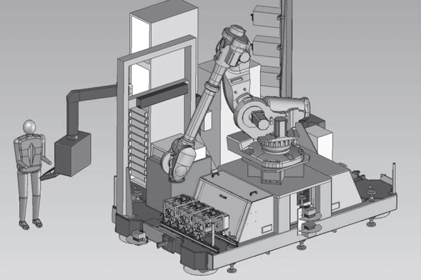
\includegraphics[width=.4\linewidth]{image1}
%}%figues de la page de garde
%
%
%\def\xxpied{%
%Cycle 02 -- Modéliser les SLCI afin de prévoir leur comportement\\
%Chapitre 3 -- \xxactivite%
%}
%
%\setcounter{secnumdepth}{5}
%%---------------------------------------------------------------------------
%
%\usepackage{pgfplots}
%\begin{document}
%
%%\chapterimage{png/Fond_Cin}
%\pagestyle{empty}


%%%%%%%% PAGE DE GARDE COURS
\ifcours
\begin{tikzpicture}[remember picture,overlay]
\node at (current page.north west)
{\begin{tikzpicture}[remember picture,overlay]
\node[anchor=north west,inner sep=0pt] at (0,0) {\includegraphics[width=\paperwidth]{\thechapterimage}};
\draw[anchor=west] (-2cm,-8cm) node [line width=2pt,rounded corners=15pt,draw=ocre,fill=white,fill opacity=0.6,inner sep=40pt]{\strut\makebox[22cm]{}};
\draw[anchor=west] (1cm,-8cm) node {\huge\sffamily\bfseries\color{black} %
\begin{minipage}{1cm}
\rotatebox{90}{\LARGE\sffamily\textsc{\color{ocre}\textbf{\xxnumpartie}}}
\end{minipage} \hfill
\begin{minipage}[c]{14cm}
\begin{titrepartie}
\begin{flushright}
\renewcommand{\baselinestretch}{1.1} 
\Large\sffamily\textsc{\textbf{\xxpartie}}
\renewcommand{\baselinestretch}{1} 
\end{flushright}
\end{titrepartie}
\end{minipage} \hfill
\begin{minipage}[c]{3.5cm}
{\large\sffamily\textsc{\textbf{\color{ocre} \discipline}}}
\end{minipage} 
 };
\end{tikzpicture}};
\end{tikzpicture}


\begin{tikzpicture}[overlay]
\node[shape=rectangle, 
      rounded corners = .25 cm,
	  draw= ocre,
	  line width=2pt, 
	  fill = ocre!10,
	  minimum width  = 2.5cm,
	  minimum height = 3cm,] at (18cm,0) {};
\node at (17.7cm,0) {\rotatebox{90}{\textbf{\Large\color{ocre}{\classe}}}};
%{};
\end{tikzpicture}

\vspace{3.5cm}

\begin{tikzpicture}[remember picture,overlay]
\draw[anchor=west] (-2cm,-6cm) node {\huge\sffamily\bfseries\color{black} %
\begin{minipage}{2cm}
\begin{center}
\LARGE\sffamily\textsc{\color{ocre}\textbf{\xxactivite}}
\end{center}
\end{minipage} \hfill
\begin{minipage}[c]{15cm}
\begin{titrechapitre}
\renewcommand{\baselinestretch}{1.1} 
\Large\sffamily\textsc{\textbf{\xxnumchapitre}}

\Large\sffamily\textsc{\textbf{\xxchapitre}}
\vspace{.5cm}

\renewcommand{\baselinestretch}{1} 
\normalsize\normalfont
\xxcompetences
\end{titrechapitre}
\end{minipage}  };
\end{tikzpicture}
\vfill

\begin{flushright}
\begin{minipage}[c]{.3\linewidth}
\begin{center}
\xxfigures
\end{center}
\end{minipage}\hfill
\begin{minipage}[c]{.6\linewidth}
\startcontents
\printcontents{}{1}{}
\end{minipage}
\end{flushright}

\begin{tikzpicture}[remember picture,overlay]
\draw[anchor=west] (4.5cm,-.7cm) node {
\begin{minipage}[c]{.2\linewidth}
\begin{flushright}

\includegraphics[width=2cm]{logoCC}
\end{flushright}
\end{minipage}
\begin{minipage}[c]{.2\linewidth}
\textsl{\xxauteur} \\
\textsl{\classe}
\end{minipage}
 };
\end{tikzpicture}
\newpage
\pagestyle{fancy}

\newpage
\pagestyle{fancy}

\else
\fi


%%%%%%%% PAGE DE GARDE TD
\iftd
%\begin{tikzpicture}[remember picture,overlay]
%\node at (current page.north west)
%{\begin{tikzpicture}[remember picture,overlay]
%\draw[anchor=west] (-2cm,-3.25cm) node [line width=2pt,rounded corners=15pt,draw=ocre,fill=white,fill opacity=0.6,inner sep=40pt]{\strut\makebox[22cm]{}};
%\draw[anchor=west] (1cm,-3.25cm) node {\huge\sffamily\bfseries\color{black} %
%\begin{minipage}{1cm}
%\rotatebox{90}{\LARGE\sffamily\textsc{\color{ocre}\textbf{\xxnumpartie}}}
%\end{minipage} \hfill
%\begin{minipage}[c]{13.5cm}
%\begin{titrepartie}
%\begin{flushright}
%\renewcommand{\baselinestretch}{1.1} 
%\Large\sffamily\textsc{\textbf{\xxpartie}}
%\renewcommand{\baselinestretch}{1} 
%\end{flushright}
%\end{titrepartie}
%\end{minipage} \hfill
%\begin{minipage}[c]{3.5cm}
%{\large\sffamily\textsc{\textbf{\color{ocre} \discipline}}}
%\end{minipage} 
% };
%\end{tikzpicture}};
%\end{tikzpicture}

%%%%%%%%%% PAGE DE GARDE TD %%%%%%%%%%%%%%%
%\begin{tikzpicture}[overlay]
%\node[shape=rectangle, 
%      rounded corners = .25 cm,
%	  draw= ocre,
%	  line width=2pt, 
%	  fill = ocre!10,
%	  minimum width  = 2.5cm,
%	  minimum height = 2.5cm,] at (18.5cm,0) {};
%\node at (17.7cm,0) {\rotatebox{90}{\textbf{\Large\color{ocre}{\classe}}}};
%%{};
%\end{tikzpicture}

% PARTIE ET CHAPITRE
%\begin{tikzpicture}[remember picture,overlay]
%\draw[anchor=west] (-1cm,-2.1cm) node {\large\sffamily\bfseries\color{black} %
%\begin{minipage}[c]{15cm}
%\begin{flushleft}
%\xxnumchapitre \\
%\xxchapitre
%\end{flushleft}
%\end{minipage}  };
%\end{tikzpicture}

% Bandeau titre exo
\begin{tikzpicture}[remember picture,overlay]
\draw[anchor=west] (-2cm,-4cm) node {\huge\sffamily\bfseries\color{black} %
\begin{minipage}{5cm}
\begin{center}
\LARGE\sffamily\color{ocre}\textbf{\textsc{\xxactivite}}

\begin{center}
\xxfigures
\end{center}

\end{center}
\end{minipage} \hfill
\begin{minipage}[c]{12cm}
\begin{titrechapitre}
\renewcommand{\baselinestretch}{1.1} 
\large\sffamily\textbf{\textsc{\xxtitreexo}}

\small\sffamily{\textbf{\textit{\color{black!70}\xxsourceexo}}}
\vspace{.5cm}

\renewcommand{\baselinestretch}{1} 
\normalsize\normalfont
\xxcompetences
\end{titrechapitre}
\end{minipage}  };
\end{tikzpicture}

\else
\fi


%%%%%%%% PAGE DE GARDE FICHE
\iffiche
\begin{tikzpicture}[remember picture,overlay]
\node at (current page.north west)
{\begin{tikzpicture}[remember picture,overlay]
\draw[anchor=west] (-2cm,-3.25cm) node [line width=2pt,rounded corners=15pt,draw=ocre,fill=white,fill opacity=0.6,inner sep=40pt]{\strut\makebox[22cm]{}};
\draw[anchor=west] (1cm,-3.25cm) node {\huge\sffamily\bfseries\color{black} %
\begin{minipage}{1cm}
\rotatebox{90}{\LARGE\sffamily\textsc{\color{ocre}\textbf{\xxnumpartie}}}
\end{minipage} \hfill
\begin{minipage}[c]{14cm}
\begin{titrepartie}
\begin{flushright}
\renewcommand{\baselinestretch}{1.1} 
\large\sffamily\textsc{\textbf{\xxpartie} \\} 

\vspace{.2cm}

\normalsize\sffamily\textsc{\textbf{\xxnumchapitre -- \xxchapitre}}
\renewcommand{\baselinestretch}{1} 
\end{flushright}
\end{titrepartie}
\end{minipage} \hfill
\begin{minipage}[c]{3.5cm}
{\large\sffamily\textsc{\textbf{\color{ocre} \discipline}}}
\end{minipage} 
 };
\end{tikzpicture}};
\end{tikzpicture}


\begin{tikzpicture}[overlay]
\node[shape=rectangle, 
      rounded corners = .25 cm,
	  draw= ocre,
	  line width=2pt, 
	  fill = ocre!10,
	  minimum width  = 2.5cm,
	  minimum height = 2.5cm,] at (18.5cm,0.5cm) {};
%	  minimum height = 2.5cm,] at (18.5cm,0cm) {};
\node at (17.7cm,0.5) {\rotatebox{90}{\textsf{\textbf{\large\color{ocre}{\classe}}}}};
%{};
\end{tikzpicture}



\else
\fi



%\vspace{4.5cm}
%\pagestyle{fancy}
%\thispagestyle{plain}
%
%\def\columnseprulecolor{\color{ocre}}
%\setlength{\columnseprule}{0.4pt} 
%
%\def\pathfig{images}




\ifprof
\else
\begin{multicols}{2}
\fi


%\section{Fauteuil dynamique de cinéma}
\section*{Présentation du système}
\setcounter{exo}{0}
\ifprof
\else
Ce concept a été inventé au Canada en 2008, et s'est étendu à toute l'Amérique du Nord avant de traverser l'Atlantique pour proposer un cinéma dynamique avec une quantité d'effets spéciaux et spatiaux. Le fauteuil dynamique de cinéma est principalement destiné à l'industrie du divertissement et de la simulation.
\fi

\subsection*{Mise en situation}
\ifprof
\else

Le siège dynamique est constitué :
\begin{itemize}
\item du dosseret qui permet d'agir directement sur la tête du spectateur afin d'amplifier la sensation d'accélération (via
l'oreille interne);%. Le point de contact entre le dosseret et la tête du spectateur est matérialisé par le point $D$ ;
\item de l'assise du siège qui permet d'obtenir un mouvement de tangage et un mouvement de roulis du spectateur.
\end{itemize}

%\begin{minipage}[c]{.48\linewidth}
%\begin{figure}[!htb]
\begin{center}
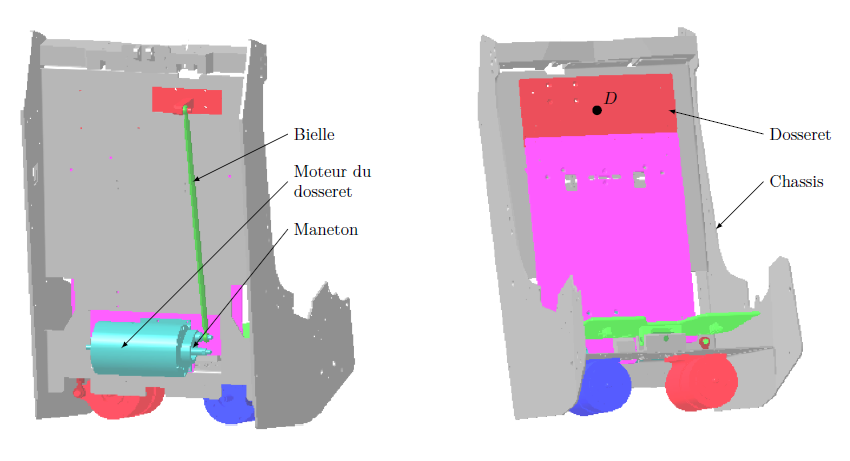
\includegraphics[width=\linewidth]{image4.png}

\textit{Dosseret \label{fig2}}
\end{center}
%\end{figure}

%\begin{figure}[!htb]
%\end{minipage}\hfill
%\begin{minipage}[c]{.48\linewidth}
%\begin{center}
%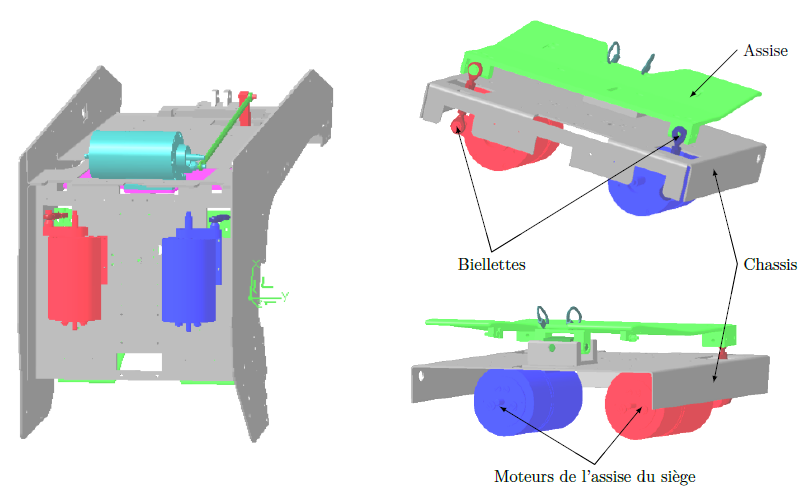
\includegraphics[width=0.9\linewidth]{image5.png}

%\textit{Assise du siège \label{fig3}}
%\end{center}
%\end{minipage}
%\end{figure}


Les trois motorisations (une pour le dosseret et deux pour l'assise)
sont composées chacune d'un moteur à courant continu à aimants
permanents et d'un réducteur de vitesse. Chaque moteur est alimenté par
un variateur de vitesse dont la structure de puissance est un hacheur.
Un capteur de courant interne au variateur est utilisé par ce dernier pour réaliser un asservissement de courant, donc implicitement de couple. Une génératrice tachymétrique accouplée
à l'axe de chaque moteur est utilisée par le variateur correspondant
pour réaliser un asservissement de vitesse. Un codeur incrémental
accouplé aussi sur l'axe de chaque moteur est utilisé par une carte à
base de microcontrôleur pour réaliser un asservissement de position, une
sortie analogique de cette carte étant reliée à l'entrée de consigne du
variateur de vitesse.
\fi
%
%\subsubsection{Étude proposée}
%
%Les accélérations procurées aux spectateurs sont un élément fondamental
%qui conditionne la conception et la réalisation de ce fauteuil dynamique
%de cinéma. Les solutions technologiques retenues répondent à cet
%objectif. Elles ne sont pas toutes abordées dans ce sujet. Quelques unes
%de celles retenues pour le fauteuil dynamique de cinéma sont étudiées
%pour valider les solutions choisies par les concepteurs vis-à-vis des
%performances attendues listées par le cahier des charges. Dans cette
%optique, il est proposé au candidat les trois études suivantes :
%
%\begin{itemize}
%\item modélisation, validation et optimisation de certains constituants
%associés à l'exigence fonctionnelle « amplifier la sensation
%d'accélération » ;
%\item validation de l'architecture de la chaine fonctionnelle réalisant
%l'exigence fonctionnelle « incliner le spectateur suivant l'axe de
%tangage et de roulis » ;
%\item synthèse globale de l'étude proposée.
%\end{itemize}


\subsection*{Exigence fonctionnelle « amplifier la sensation
d'accélération »}
\ifprof
\else

\begin{obj}
Proposer un modèle de comportement des éléments réalisant l'exigence
fonctionnelle « amplifier la sensation d'accélération » puis valider les
performances attendues listées par le cahier des charges.
\end{obj}

\textbf{Exigence : amplifier la sensation d'accélération}
\begin{itemize}
\item  Précision statique de la boucle d'asservissement de position :
\begin{itemize}
\item erreur statique de position $<1\%$;
\item erreur statique de traînage $<1\%$; 
\item erreur statique d'accélération $<1\%$ .
\end{itemize}
\item Rapidité pour un échelon de consigne d'accélération :
\begin{itemize}
\item temps de montée de 0 à 100\% de la consigne~$<\SI{5}{ms}$;
\item dépassement $<20\%$.
\end{itemize}
\end{itemize}
\fi

%%\begin{table}[!htb]
% %\centering
% \begin{center}
%    \begin{tabular}{|p{0.2\linewidth}|p{0.35\linewidth}|p{0.35\linewidth}|}
%    \hline
%    \textbf{Exigence} & \textbf{Critères d'appréciation} & \textbf{Niveau} \\
%    \hline
%    Amplifier la sensation d'accélération & Précision statique de la boucle d'asservissement de position & \multicolumn{1}{r|}{} \\
%          & Erreur statique de position  &$<1\%$\\
%          & Erreur statique de traînage  & $<1\%$ \\
%          & Erreur statique d'accélération & $<1\%$ \\
%\cline{2-3}          & Rapidité pour un échelon de consigne d'accélération &  \\
%          & Temps de montée de 0 à 100\% de la consigne  & $<\SI{5}{ms}$ \\
%          & Dépassement & $<20\%$ \\
%%\cline{2-3}          & Accélération maximale du point $D$ de la tête du spectateur situé à 85 mm au-dessus de l'axe de rotation du dosseret & $\SI{6}{m. s^{-2}}(\SI{0,6}{g})< a_{\text{max}} < \SI{7}{m. s^{-2}}(\SI{0,7}{g})$ \\
%\hline
%    \end{tabular}%
%    
%\textit{Extrait du cahier des charges associé à l'exigence fonctionnelle « Amplifier la sensation d'accélération » \\  réalisée par le dosseret \label{tab:4}}%
% \end{center}
% %\end{table}%

%%\FloatBarrier
%\subsection*{Notations et hypothèses}

%Le schéma multi physique et le  le schéma-blocs modélisant l'asservissement de position du
%dosseret sont fournis figure ci-dessous.

%Le  schéma-blocs modélisant l'asservissement global e position du dosseret est fourni en fin de sujet.
%\textbf{Notations : }
%
%\begin{center}
%    \begin{tabular}{|p{0.1\linewidth}|p{0.35\linewidth}|p{0.1\linewidth}|p{0.1\linewidth}|}
%    \hline
%      & \textbf{Description} & \textbf{Variable temporelle} & {\textbf{Unité}} \\
%    \hline
%    $\theta_{Cd}(p)$ & consigne de position du dosseret & {$\theta_{Cd}(t)$} &  {rad} \\
%    \hline
%    $\theta_{C}(p)$ & consigne de position de l'axe moteur &  {$\theta_{C}(t)$} &  {rad} \\
%    \hline
%    $\theta_{}(p)$ & position de l'axe moteur &  {$\theta_{}(t)$} &  {rad} \\
%    \hline
%    $\theta_{r}(p)$ & position de l'axe de sortie du réducteur &  {$\theta_{r}(t)$} &  {rad} \\
%    \hline
%    $\theta_{d}(p)$ & position du dosseret &  {$\theta_{d}(t)$} &  {rad} \\
%    \hline
%    $N_{\text{Codeur}}(p)$ & valeur  numérique  issue du comptage  incrémental &  {$N_{\text{Codeur}}(t)$} &  \\
%    \hline
%    $r$ & rapport de transmission du réducteur &       &  \\
%    \hline
%    $K_c$ & gain du mécanisme  de la transformation de mouvement du dosseret &       &  \\
%    \hline
%    \end{tabular}%
%\end{center}

%%\begin{figure}[!htb]
%\begin{center}
%\rotatebox{270}{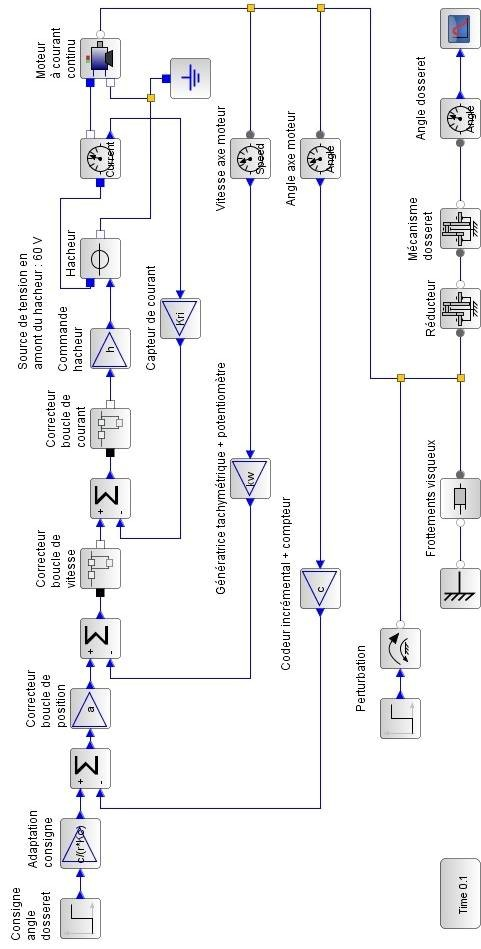
\includegraphics[height=\linewidth]{image6.jpeg}}
%
%\vspace{.5cm}
%
%\textit{Schéma multi physique de l'asservissement du dosseret \label{fig5}}
%\end{center}
%%\end{figure}

%\begin{figure}[!htb]

%\end{figure}
%%\FloatBarrier

%
%\begin{center}
%\begin{tabular}{|p{0.08\linewidth}|p{0.3\linewidth}|p{0.1\linewidth}|p{0.1\linewidth}|}
%    \hline
%   & \textbf{Description} & \textbf{Variable temporelle} &  \textbf{Unité}\\
%    \hline
%    \textit{c} & gain du codeur incrémental &       & $\text{rad}^{-1}$ \\
%    \hline
%    \textit{a} & gain proportionnel du correcteur de l'asservissement de position &       & V \\
%    \hline
%$U_{c\Omega}(p)$ & image de la consigne de vitesse de l'axe moteur & $U_{c\Omega}(t)$ & V \\
%    \hline
%$\Omega(p)$ & vitesse de l'axe moteur & $\Omega(t)$ & $\text{rad s}^{-1}$ \\
%    \hline
%$C_{\Omega}(p)$ & correcteur de l'asservissement de vitesse &       &  \\
%    \hline
%$I_c(p)$ & image de la consigne de courant & $i_c(t)$ & V \\
%    \hline
%$C_I(p)$ & correcteur de l'asservissement de courant &       &  \\
%    \hline
%$h$ & gain du hacheur &       &  \\
%    \hline
%$K_{rI}$ & gain du capteur de courant &       &  \\
%    \hline
%$U(p)$ & tension  d'alimentation du moteur & $u(t)$ & V \\
%    \hline
%$E(p)$ & force électromotrice du moteur & $e(t)$ & V \\
%    \hline
%$I(p)$ & courant dans l'induit du moteur & $i(t)$ & A \\
%    \hline
%$C_M(p)$ & couple moteur & $c_M(t)$ & $\text{Nm}$ \\
%    \hline
%$C_R(p)$ & couple résistant perturbateur & $c_R(t)$ & $\text{Nm}$ \\
%    \hline
%$L$ & inductance du circuit  d'induit  du moteur &       &  \\
%    \hline
%$R$ & résistance  du circuit  d'induit  du moteur &       &  \\
%    \hline
%$K_{\Omega}$ & gain de la génératrice tachymétrique &       & $\text{V}\cdot \text{s}\cdot \text{rad}^{-1}$ \\
%    \hline
%$K$ & gain de la constante de couple ou de la constante de force électromotrice &       &  \\
%    \hline
%$J$ & moment  d'inertie  de l'ensemble  en mouvement, ramené  au  niveau  de l'axe moteur &       &  \\
%    \hline
%$f$ & coefficient de frottements visqueux équivalent pour l'ensemble en mouvement &       &  \\
%\hline
%\end{tabular}
%\end{center}

%
%\textbf{Données}
%
%
%\begin{multicols}{2}
%\begin{itemize}
%\item $K = \SI{0,115}{N.m.A^{-1}}$ ($\text{V\,s\,rad}^{-1})$;
%\item $R = \SI{1}{\Omega}$;
%\item $L = \SI{1,1}{mH}$;
%\item $K_{rI}= \SI{0,5}{V. A^{-1}}$
%\item $h = 6$;
%\item $r = 1/50$;
%\item $f = \SI{4e-4}{N.m.s.rad^{-1}}$;
%\item $J=\SI{0,16e-3}{kg.m^2}$.
%\end{itemize}
%\end{multicols}
%**********************

%\begin{longtable}[]{@{}ll@{}}
%\toprule
%\begin{minipage}[t]{0.48\columnwidth}\raggedright\strut
%\emph{K = 0,115 N.m.A\textsuperscript{-1}}
%
%\emph{R = 1 $\Omega$}
%
%\emph{L = 1,1mH}
%
%\emph{K\textsubscript{rI}= 0,5 V. A\textsuperscript{-1}}\strut
%\end{minipage} & \begin{minipage}[t]{0.48\columnwidth}\raggedright\strut
%\emph{h = 6}
%
%\emph{r = 1/50}
%
%\emph{f = 4.10\textsuperscript{-4} N.m.s.rad\textsuperscript{-1}}
%
%$J=0,16.10^{-3} kg.m^2$ \strut
%\end{minipage}\tabularnewline
%\bottomrule
%\end{longtable}

%**************
%Correcteur de courant :
%\(C_{I}\left( p \right) = k_{2}\left( 1 + \frac{1}{T_{2}p} \right)\)
%avec \emph{k\textsubscript{2} = 5} et \emph{T\textsubscript{2} = 0,3 ms}.
%
%Correcteur de vitesse :
%\(C_{\Omega}\left( p \right) = k_{1}\left( 1 + \frac{1}{T_{1}p} \right)\)
%avec \emph{k\textsubscript{1} = 20}.

%%\textbf{Hypothèses}
%\newpage
%
%\begin{hypo}~\\
%\begin{itemize}
%\item  La période d'échantillonnage est suffisamment faible pour être
%négligeable devant la dynamique globale du système et les différentes
%variables sont donc toutes considérées comme des fonctions continues du
%temps.
%\item Le temps de réponse du hacheur est considéré négligeable dans l'étude.
%\item Les conditions de Heaviside sont vérifiées.
%\end{itemize}
%\end{hypo}

%\subsection{Comportement cinématique du mécanisme de transformation de mouvement du dosseret}
%
%\begin{obj}
%Valider la linéarité du comportement du mécanisme de transformation de
%mouvement du dosseret en établissant la loi de comportement
%cinématique.
%\end{obj}
%%
%%Le modèle cinématique de la transformation de mouvement du dosseret est
%%fourni figure \ref{fig8}.
%%
%%
%%\subparagraph{}\textit{À l'aide d'une fermeture géométrique, exprimer littéralement l'angle
%%  \emph{$\theta$\textsubscript{d}} en fonction de l'angle
%%  \emph{$\theta$\textsubscript{r}}. Mettre l'expression sous la forme :
%%\[\cos\theta_{d}\left( E + F\cos\theta_{r} \right) + \sin\theta_{d}\left( G + F\sin\theta_{r} \right) = H + \left(I\cos\theta_{r} + J\sin\theta_{r} \right)\].}
%
%Une simulation numérique a permis d'obtenir le tracé représenté sur la
%figure suivante, illustrant l'évolution de l'angle du dosseret en fonction de l'angle du moteur. 
%Afin d'obtenir un modèle linéaire de la caractéristique
%\(\theta_{d} = f\left( \theta_{r} \right)\), l'étude se fait autour de
%son point de fonctionnement statique pour de petites variations.
%
%\begin{center}
%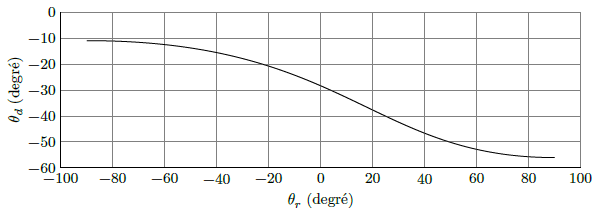
\includegraphics[width=1.0\linewidth]{image10.png}
%
%\textit{Représentation de l'équation de fermeture géométrique\label{fig9}}
%\end{center}
%%\end{figure}
%
%\subparagraph{}\textit{Déterminer par linéarisation autour du point de fonctionnement
%  \(\theta_{r} = 0\), la valeur numérique du gain dynamique
%  \emph{K\textsubscript{c}} de la transformation de mouvement du
%  dosseret.}
%  
%
%
%%\begin{figure}[!htb]
%\begin{center}
%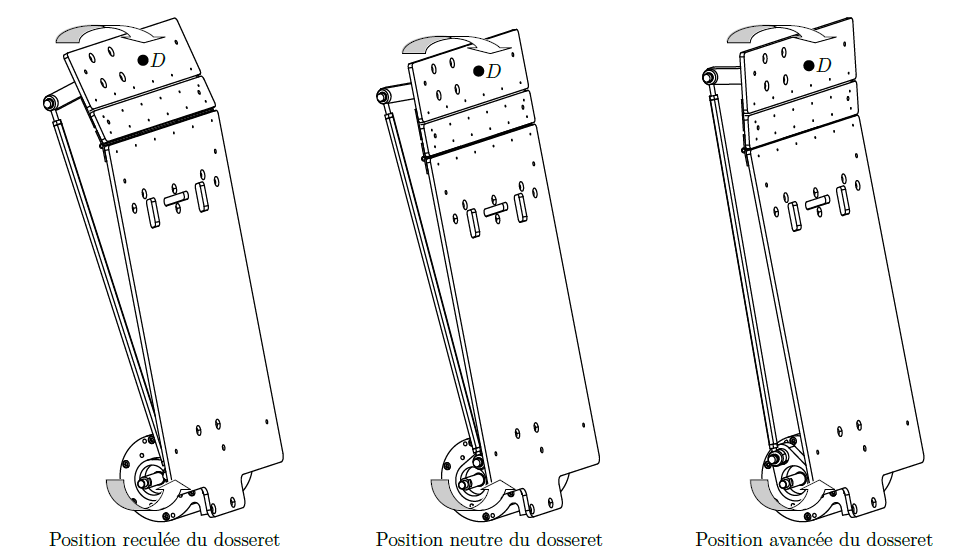
\includegraphics[width=.8\linewidth]{image8.png}

%\textit{Mécanisme de transformation de mouvement du dosseret\label{fig7}}
%\end{center}
%%\end{figure}
%
%
%%\begin{figure}[!htb]
%\begin{center}

%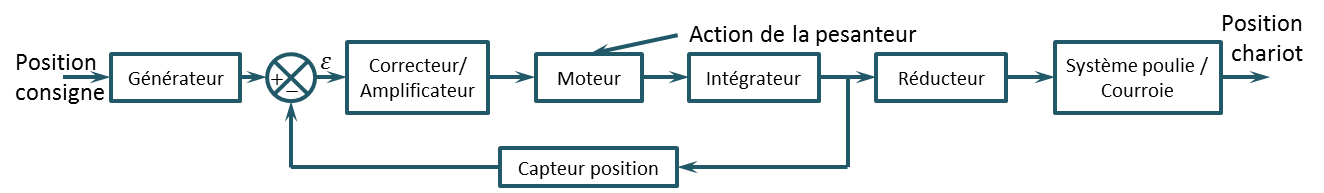
\includegraphics[width=1.0\linewidth,angle=90]{image9.png}

%\textit{Modèle cinématique de la transformation de mouvement
%du dosseret \label{fig8}}
%\end{center}
%%\end{figure}

%\begin{figure}[!htb]



%\subsection{Comportement du codeur incrémental et de la
%génératrice tachymétrique}
%
%\begin{obj}
%Établir un modèle de comportement du codeur incrémental et de la
%génératrice tachymétrique.
%\end{obj}
%
%Le moteur AXEM a pour référence F12M4. Il est alimenté par une carte
%variateur de vitesse RTS 10-20-60 (PARVEX) alimentée sous \SI{60}{V} DC et
%pouvant délivrer \SI{20}{A} pendant \SI{2}{s}, avec un courant nominal de \SI{10}{A}.
%
%Ce dernier comprend les boucles d'asservissement de vitesse et de
%courant. Sur l'arbre moteur sont montés une génératrice tachymétrique et
%un codeur incrémental $\SI{250}{points.tour^{-1}}$. Le comptage incrémental est
%effectué sur le front montant d'une des deux voies. La génératrice
%tachymétrique est raccordée à l'entrée de retour vitesse du variateur.
%Un réglage par potentiomètre présent dans le variateur est effectué pour
%obtenir une tension de \SI{5}{V} au niveau du comparateur de l'asservissement
%de vitesse lorsque la fréquence de rotation du moteur est égale à $\SI{3000}{tr. min^{-1}}$.
%
%\subparagraph{}\textit{En tenant compte des informations précédentes, calculer la valeur
%  numérique de $c$ et de $K_\Omega$ (schéma-blocs précédent).}

%\newpage
\subsection*{Comportement de l'ensemble variateur et moteur du dosseret}

\begin{obj} ~\\
%Valider un modèle simplifié de l'asservissement de position de l'axe
%moteur afin d'analyser les paramètres influant sur la précision et
%proposer une amélioration du système.
%
%Pour cela, il faut :
\begin{itemize}
\item Établir un modèle simplifié de l'asservissement de courant.
\item Établir un modèle simplifié de l'asservissement de vitesse.
\item Analyser la précision de l'asservissement de position.
\end{itemize}
\end{obj}
%
%
%\subsubsection*{Modélisation de l'asservissement du courant}
%
%L'étude suivante consiste à vérifier la validité de la simplification du
%modèle de la boucle d'asservissement du courant (passage du modèle initial au modèle simplifié).
%
%%\begin{figure}[!htb]
%\begin{center}
%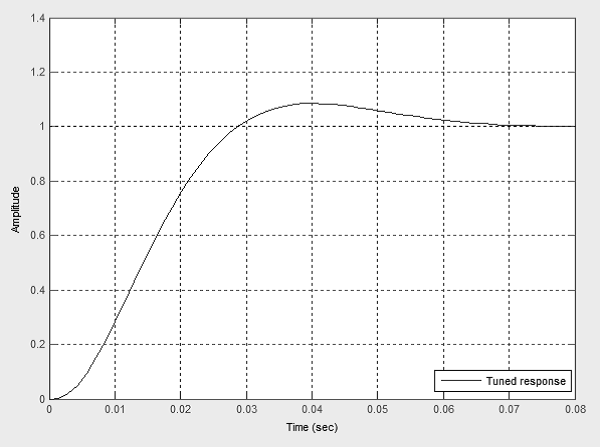
\includegraphics[width=1.0\linewidth]{image11.png}
%
%\textit{Modèle initial de la boucle d'asservissement de courant. \label{fig10}}
%\end{center}
%%\end{figure}
%
%
%%\begin{figure}[!htb]
%\begin{center}
%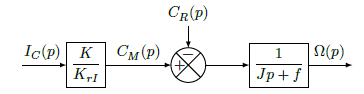
\includegraphics[width=\linewidth]{image12.png}
%
%\textit{Modèle simplifié de la boucle d'asservissement de courant. \label{fig11}}
%\end{center}
%%\end{figure}
%
%
%Pour le modèle initial
% %de la figure \ref{fig10}
%  lorsque C\emph{\textsubscript{R}} (p) =0, la fonction de transfert s'écrit :
%
%\[\frac{\Omega(p)}{I_{c}(p)} = \frac{Kk_{2}hT_{2}p + Kk_{2}h}{T_{2}\text{LJ}p^{3} + \left( T_{2}\left( Lf + RJ \right) + k_{2}hk_{\text{rI}}T_{2}J \right)p + \left( T_{2}\left( Rf + K \right) + k_{2}hk_{\text{rI}}\left( T_{2}f + J \right) \right)p + k_{2}hk_{\text{rI}}f}.\]
%
%À l'aide d'un logiciel de simulation, une comparaison du comportement de la vitesse en sortie des deux modèles a été effectuée (figure suivante)%\ref{fig12})
% et ce pour un échelon unitaire de consigne de courant appliqué en entrée.
%
%%\begin{figure}[!htb]
%\begin{center}
%
%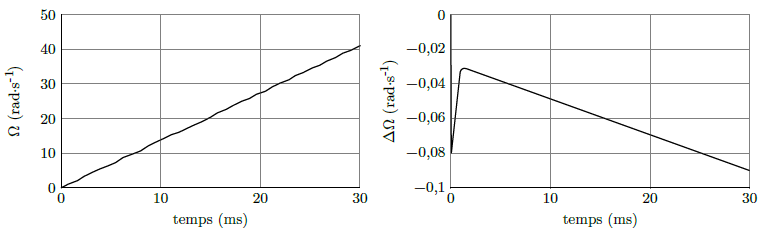
\includegraphics[width=1.0\linewidth]{image13.png}
%\footnotesize \textit{Vitesse de l'axe moteur pour le modèle initial ($\Omega_{\text{initial}}$) et écart entre le modèle initial et le modèle simplifié pour la vitesse de l'axe moteur ($\Delta \Omega=\Omega_{\text{initial}}-\Omega_{\text{simplifie}}$)}
%\normalsize
%
%\end{center}
%%\end{figure}
%
%
%
%\subparagraph{}\textit{Pour chacun des deux modèles (initial et simplifié), quelle est la
%  valeur finale de $\Omega(t)$ lorsque $i_c(t)$ est un
%  échelon unitaire ? À l'aide de ces résultats et des relevés issus de
%  la simulation dans le régime transitoire, conclure quant à la validité
%  de la simplification du modèle sachant que chaque sollicitation du
%  dosseret a une durée d'environ \SI{30}{ms}.}
%
%
%


%%\FloatBarrier
\subsubsection*{Modélisation de l'asservissement de vitesse}

\textbf{NE PAS TRAITER LES QUESTIONS 1 à 3.}
\ifprof
\else

\begin{rem}
Les 3 premières questions n'ont pas vraiment d'intérêt. Je les ai laissées car elles apparaissaient dans le sujet initial.
\end{rem}

L'étude suivante consiste à obtenir un modèle simplifié de la boucle
d'asservissement de vitesse (figure suivante) au regard des réglages effectués
et de l'influence d'une perturbation de type échelon sur le dosseret. En
effet, vu la courte durée des sollicitations, la perturbation sur le
dosseret, dont l'origine peut être une action du spectateur sur ses
muscles cervicaux, peut être modélisée par un échelon.

%\begin{figure}[!htb]
\begin{center}
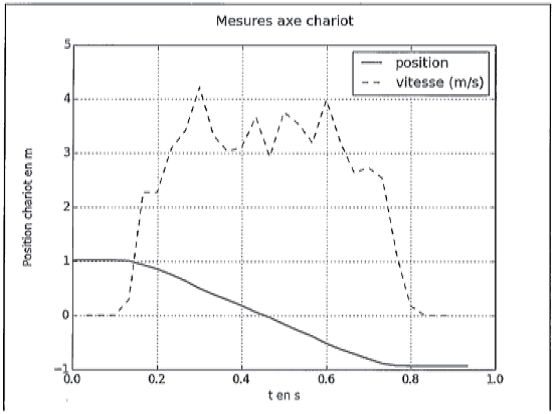
\includegraphics[width=1.0\linewidth]{image14.png}
\textit{Modèle de la boucle d'asservissement de vitesse \label{fig13}}
\end{center}
%\end{figure}

 On a \(C_{\Omega}\left( p \right) = k_{1}\left( 1 + \dfrac{1}{T_{1}p} \right)\). De plus : 
$K = \SI{0,115}{N.m.A^{-1}}$;
$R = \SI{1}{\Omega}$;
$L = \SI{1,1}{mH}$;
$K_{rI}= \SI{0,5}{V. A^{-1}}$;
%	h = 6
$r = 1/50$;
$f = \SI{4.1e-4}{N.m.s.rad^{-1}}$;
$J=\SI{0,16e-3}{kg.m^{2}}$.

 
 
 
 \fi
 

\subparagraph{}\textit{Exprimer la fonction de transfert de la boucle de vitesse
  \(H_{\Omega}\left( p \right) = \Omega(p)/U_{C\Omega}(p)\), lorsque
  \(C_{R}\left( p \right) = 0\). Le résultat sera mis sous une forme canonique.}

\ifprof
\begin{corrige}~\\

$H_{\Omega}(p)=\dfrac{k_{1}\left( 1 + \dfrac{1}{T_{1}p} \right)\dfrac{K}{K_{rI}}\dfrac{1}{Jp+f}}{1+ K_{\Omega}k_{1}\left( 1 +\dfrac{1}{T_{1}p} \right)\dfrac{K}{K_{rI}}\dfrac{1}{Jp+f}}$
$=\dfrac{k_{1}\left( 1 + T_{1}p \right)K}{T_{1}p K_{rI}\left(Jp+f\right) + K_{\Omega}k_{1}\left(1+ T_{1}p\right) K}$

~\\

$=\dfrac{\dfrac{Kk_{1}}{K_{\Omega}k_{1}K}\left( 1 + T_{1}p \right)}{\dfrac{T_{1} K_{rI}J}{K_{\Omega}k_{1}K}p^2+\left(\dfrac{fT_{1} K_{rI}}{K_{\Omega}k_{1}K}+\dfrac{K_{\Omega}k_{1}T_{1}K}{K_{\Omega}k_{1}K}\right)p + 1 }$
$H_{\Omega}(p)=\dfrac{\dfrac{1}{K_{\Omega}}\left( 1 + T_{1}p \right)}{\dfrac{T_{1} K_{rI}J}{K_{\Omega}k_{1}K}p^2+\left(\dfrac{f K_{rI}}{K_{\Omega}k_{1}K}+1\right)T_{1}p + 1 }$

\end{corrige}
\else
\fi

\subparagraph{}\textit{$T_1$ étant égal à $J/f$, montrer alors que
  la fonction de transfert en boucle fermée peut se mettre sous la forme
  \(\dfrac{b}{\tau p + 1}\). Calculer les valeurs numériques des termes
  \emph{b} et \emph{$\tau$}.}

\ifprof
\begin{corrige}~\\

\footnotesize

On a 
$H_{\Omega}(p)=\dfrac{\dfrac{1}{K_{\Omega}}\left( 1 + \dfrac{J}{f}p \right)}{\dfrac{\dfrac{J}{f} K_{rI}J}{K_{\Omega}k_{1}K}p^2+\left(\dfrac{f K_{rI}}{K_{\Omega}k_{1}K}+1\right)\dfrac{J}{f}p + 1 }$
$=\dfrac{\left( f + Jp \right)}{\dfrac{ K_{rI}J^2}{k_{1}K}p^2+\left(\dfrac{f K_{rI}}{k_{1}K}+K_{\Omega}\right)Jp + fK_{\Omega}}$

$=\dfrac{\left( f + Jp \right)k_{1}K}{ K_{rI}J^2p^2+\left(f K_{rI}+K_{\Omega}k_{1}K\right)Jp + fK_{\Omega}k_{1}K}$


On a :
$\Delta =\left(f K_{rI}+K_{\Omega}k_{1}K\right)^2J^2 -4 fK_{\Omega}k_{1}KK_{rI}J^2 $ 
$=\left(f^2 K_{rI}^2+K_{\Omega}^2k_{1}^2K^2+2f K_{rI}K_{\Omega}k_{1}K\right)J^2 -4 fK_{\Omega}k_{1}KK_{rI}J^2 $

$=\left(f^2 K_{rI}^2+K_{\Omega}^2k_{1}^2K^2-2f K_{rI}K_{\Omega}k_{1}K\right)J^2  $
$=\left(f K_{rI}-K_{\Omega}k_{1}K\right)^2J^2  $

On a donc 

$p_{12} = \dfrac{-\left(f K_{rI}+K_{\Omega}k_{1}K\right)J \pm \left(f K_{rI}-K_{\Omega}k_{1}K\right)J}{2 K_{rI}J^2}$, 

$p_{1} = \dfrac{-fJ K_{rI}-K_{\Omega}k_{1}KJ + fJ K_{rI}-K_{\Omega}k_{1}KJ}{2 K_{rI}J^2}$
$= -\dfrac{K_{\Omega}k_{1}K }{ K_{rI}J}$, 
$p_{2} = \dfrac{-fJ K_{rI}-K_{\Omega}k_{1}KJ -fJ K_{rI}+K_{\Omega}k_{1}KJ}{2 K_{rI}J^2}= -\dfrac{f }{J}$.

On a donc 

$H_{\Omega}(p)=\dfrac{J\left( \dfrac{f}{J} + p \right)k_{1}K}{\left(p+\dfrac{f }{J} \right)\left(p+\dfrac{K_{\Omega}k_{1}K }{ K_{rI}J} \right)}=\dfrac{Jk_{1}K}{p+\dfrac{K_{\Omega}k_{1}K }{ K_{rI}J} }$
$=\dfrac{\dfrac{ K_{rI}J^2}{K_{\Omega} } }{\dfrac{ K_{rI}J}{K_{\Omega}k_{1}K }p+1 }$

On a donc $b=\dfrac{ K_{rI}J^2}{K_{\Omega} }$ et $\tau =\dfrac{ K_{rI}J}{K_{\Omega}k_{1}K }$.

\normalsize
Autre solution : $b=\dfrac{1}{K_{\Omega}} = 20 \pi = \SI{62,8}{rad.s{-1}V^{-1}}$ et $\tau=\dfrac{K_{ri}J}{k_1KK_{\Omega}}=\SI{2,17e-3}{s}$.


\end{corrige}
\else
\fi

\subparagraph{}\textit{En déduire, à l'aide de la figure précédente, $\theta(p)/C_R(p)$
  lorsque $\theta_C(p)=0$. Calculer ensuite la valeur finale
  de $\theta(t)$ lorsque $c_R(t)$ est un échelon unitaire. %*******
  Conclure quant à l'action, en régime permanent, du correcteur
  proportionnel et intégral sur les effets d'une perturbation
  $c_R(t)$ de type échelon.}

\ifprof
\begin{corrige}~\\

\begin{center}
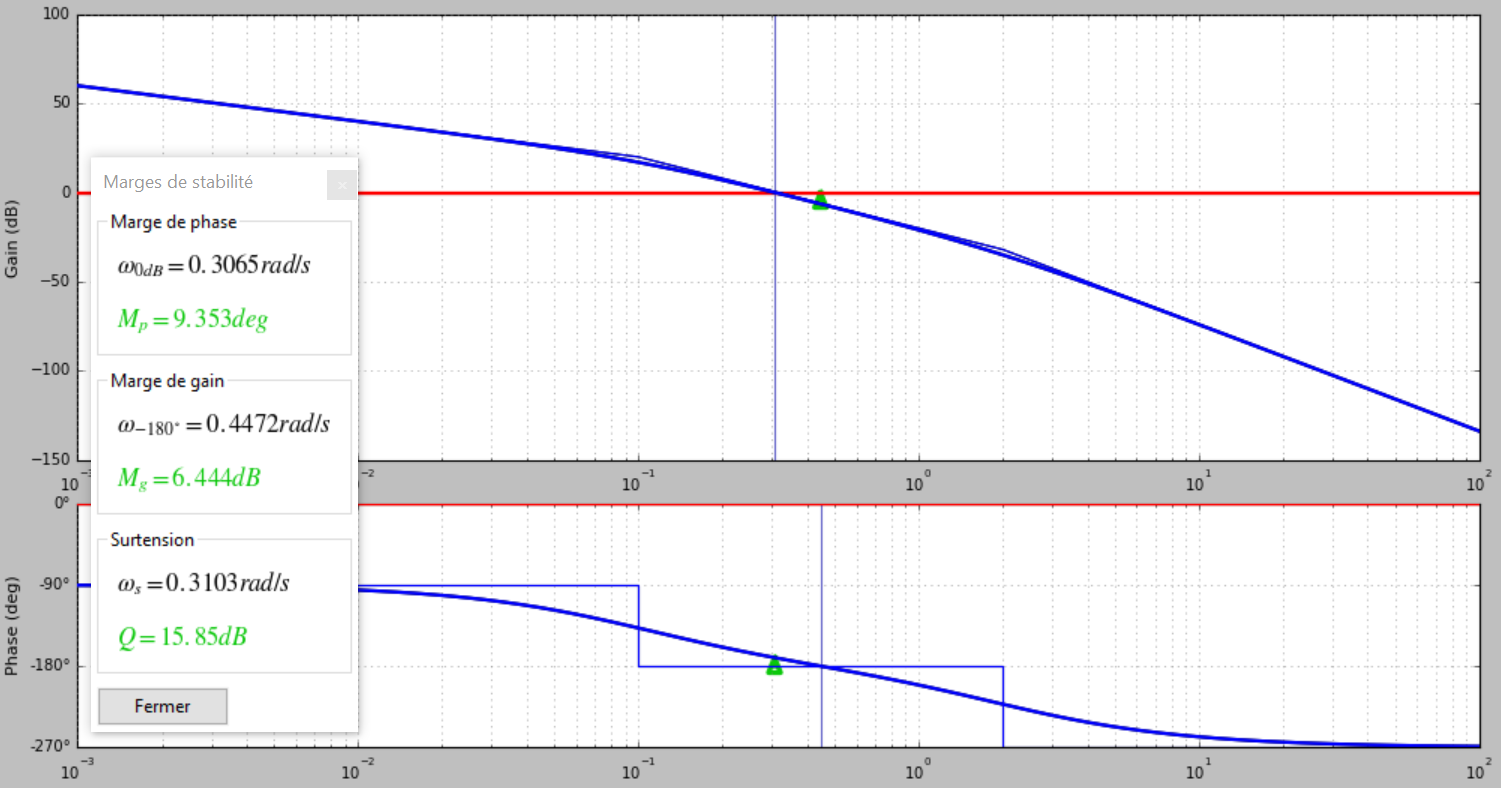
\includegraphics[width=\linewidth]{cor_01.png}
\end{center}

$\dfrac{\theta(p)}{C_r(p)}=\dfrac{1}{C_{\Omega}(p)\dfrac{K}{K_{ri}}}\dfrac{\dfrac{b}{1+\tau p}\dfrac{1}{p}}{1+\dfrac{abc}{1+\tau p}\dfrac{1}{p}}$ 
$=\dfrac{1}{ k_{1}\left( 1 + \dfrac{1}{T_{1}p} \right)\dfrac{K}{K_{ri}}}\dfrac{\dfrac{b}{1+\tau p}\dfrac{1}{p}}{1+\dfrac{abc}{1+\tau p}\dfrac{1}{p}}$

$=\dfrac{T_{1}K_{ri}p}{ k_{1}\left( T_{1}p + 1 \right)K}\cdot \dfrac{b}{p\left(1+\tau p \right)+abc}$

et $\lim\limits_{t\to\infty} \theta(t) = 1$.
\end{corrige}
\else
\fi

\subsubsection*{Modélisation de la boucle d'asservissement de position}
\ifprof
\else

Après toutes les simplifications précédentes, est obtenu le modèle de la
figure suivante où seul le comportement en réponse à la consigne
$\theta$\textsubscript{C} est abordé.


%\begin{figure}[!htb]
\begin{center}
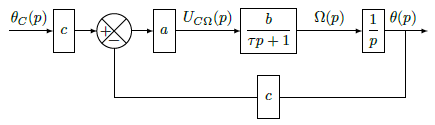
\includegraphics[width=\linewidth]{image15.png}

\textit{Modèle simplifié de la boucle d'asservissement de
position \label{fig14}}
\end{center}
%\end{figure}

\fi


\subparagraph{}\textit{Exprimer la fonction de transfert $\theta(p)/\theta_C(p)$.
  Déterminer ensuite la valeur numérique de $a$ pour avoir un facteur
  d'amortissement égal à $0,7$. Justifier le choix de ce facteur
  d'amortissement. (Pour ce calcul et les calculs suivants prendre $b =
  \SI{63}{rad\cdot s^{-1}\cdot V^{-1}}$, $\tau= \SI{2,2}{ms}$, $c = \SI{40}{rad^{-1}}$.)}

\ifprof
\begin{corrige}~\\

On a $\dfrac{\theta(p)}{\theta_C(p)}=c\dfrac{\dfrac{ab}{p\left( \tau p + 1\right)}}{1+\dfrac{abc}{p\left( \tau p + 1\right)}}$
$=\dfrac{{abc}}{p\left( \tau p + 1\right)+{abc}}=\dfrac{1}{ \dfrac{\tau}{abc} p^2 + \dfrac{p}{abc}+1}$.

On a $\omega_0 = \sqrt{abc/\tau}$ et $\dfrac{2\xi}{\omega_0}=\dfrac{1}{abc}$ et 
$\xi=\dfrac{1}{2\sqrt{abc\tau}}$. 
En conséquence, ${a}=\dfrac{1}{4bc\tau\xi^2}=0,092$. (On prend $\xi=0,7$ car cela correspond au temps de réponse le plus rapide pour un second ordre.)
\end{corrige}
\else
\fi
  
%\subparagraph{}\textit{Tracer le diagramme de Bode de la fonction de le fonction de transfert en boucle ouverte. Quel que soit le résultat de la partie précédente, on prendra $a=\SI{0,1}{V}$.}

\subsection*{Analyse de la précision du système}
\ifprof
\else

Un aspect important pour la simulation sensorielle du siège dynamique
est la capacité du système à reproduire fidèlement la consigne de
position issue du programme de simulation sensorielle du siège
dynamique. Dans un premier temps, l'étude se limite à la précision
statique en utilisant le modèle défini à la figure précédente. L'erreur
représente la différence entre l'entrée $\theta_C(t)$ et la
sortie $\theta(t)$ et est définie par la variable $\mu(t) = \theta_C(t)-\theta(t)$.
\fi

%\textbf{Indication : } l'erreur d'accélération est déterminée suite à une entrée de type
%accélération ($\theta_C(t)=t^2\cdot \dfrac{u(t)}{2}$, $\theta_C(p)=\dfrac{1}{p^3}$.

\subparagraph{}\textit{ Exprimer dans un premier temps $\mu(p)$ en fonction de
  $\theta_C(p)$, puis déterminer de façon littérale et numérique
  l'erreur de position $\mu_p$, l'erreur de trainage
  $\mu_v$ et l'erreur en accélération $\mu_a$.
  Conclure quant à la précision statique du système suite aux
  différentes consignes $\theta_C(p)$ de type échelon, rampe et
  accélération.}

\ifprof
\begin{corrige}
On a $\mu(p)=\dfrac{\theta_c(p)}{1+\dfrac{abc}{p\left( 1+\tau p\right)}}=\dfrac{p\left( 1+\tau p\right)}{p\left( 1+\tau p\right)+abc}\theta_c(p)$ $=\dfrac{p\left( 1+\tau p\right)}{p\left( 1+\tau p\right)+abc}\theta_c(p)$.

La FTBO est de classe 1 et de gain $K_{\text{BO}}={abc}$ on a donc : 
\begin{itemize}
\item pour une entrée échelon, $\mu_p = 0$;
\item pour une entrée rampe, $\mu_v = \dfrac{1}{abc}$;
\item pour une entrée accélération, $\mu_a = \infty$.
\end{itemize}
\end{corrige}
\else
\fi

\subsection*{Validation et optimisation de la performance simulée en
accélération du dosseret}

\begin{obj}
Valider la performance simulée en accélération au regard du cahier des
charges fonctionnel.
\end{obj}
%
%Un logiciel de simulation permet d'obtenir la courbe de la vitesse angulaire maximale \({\dot{\theta}}_{d}\ \) ainsi que celle de l'accélération angulaire maximale
%\({\ddot{\theta}}_{d}\ \)(figure suivante) du dosseret. Ces deux courbes sont tracées sur une durée de 30 ms lors du démarrage du moteur (au-delà de  ce temps le moteur atteint sa vitesse nominale).
%
%%\begin{figure}[!htb]
%\begin{center}
%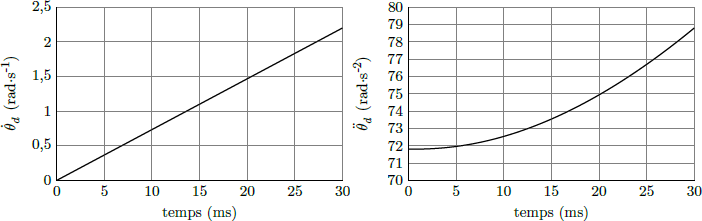
\includegraphics[width=1.0\linewidth]{image16.png}
%\textit{Vitesse et accélération angulaires en fonction du
%temps \label{fig15}}
%\end{center}
%%\end{figure}


%
%\subparagraph{}\textit{Déterminer, à partir du paramétrage donné figure \ref{fig8}, l'expression
%  littérale au point $D$ (représentant le point de contact avec la tête du
%  spectateur) du vecteur accélération
%  \({\overrightarrow{\Gamma}}_{D \in \text{dosseret}/\text{chassis}}\). Calculer
%  numériquement la norme de ce vecteur accélération au point $D$
%  correspondant à la valeur maximale de \({\ddot{\theta}}_{d}\).}
%  
%\subparagraph{}\textit{Conclure quant au respect du nombre de g du cahier des charges (tableau \ref{tab:4}) vis-à-vis des accélérations simulées produites par le dosseret du
%  siège dynamique de cinéma.}
%  

\ifprof
\else

La figure suivante représente la structure d'une correction par anticipation
qui permet d'améliorer la précision statique du système

 %\begin{figure}[!htb]
\begin{center}
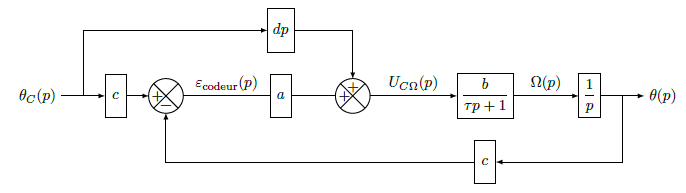
\includegraphics[width=1.0\linewidth]{image17.png}
\textit{Structure avec anticipation \label{fig16}}
\end{center}
%\end{figure}
\fi

\subparagraph{\label{q13}}\textit{Déterminer l'erreur de position $\mu$\emph{\textsubscript{p}} puis
  l'erreur de traînage $\mu$\emph{\textsubscript{v}}. Conclure sur l'erreur
  de position au regard du cahier des charges.}
\ifprof
\begin{corrige} ~\\

On a 
$\varepsilon_{\text{codeur}}(p)=c\theta_c(p)-c\theta(p)$ 

$=c\theta_c(p)-\dfrac{bc}{p\left(\tau p + 1 \right)}U_{C \Omega }(p)$
 $=c\theta_c(p)-\dfrac{bc}{p\left(\tau p + 1 \right)}\left( \theta_C(p) dp + a \varepsilon_{\text{codeur}}(p) \right)$

$\Leftrightarrow \varepsilon_{\text{codeur}}(p)\left(1+\dfrac{abc}{p\left(\tau p + 1 \right)}\right) = \theta_C(p)  \left(c-\dfrac{bcd}{\tau p + 1 } \right)$

$\Leftrightarrow \varepsilon_{\text{codeur}}(p)\left(1+\dfrac{abc}{p\left(\tau p + 1 \right)}\right) = \theta_C(p)  c \dfrac{\tau p + 1 -bd}{\tau p + 1 } $

$\Leftrightarrow \varepsilon_{\text{codeur}}(p) = \theta_C(p)  cp \dfrac{\tau p + 1 -bd}{p\left(\tau p + 1 \right)+abc} $

On a alors : 
\begin{itemize}
\item $\mu_p=\lim\limits_{p\to0}  p\dfrac{1}{p}  cp \dfrac{\tau p + 1 -bd}{p\left(\tau p + 1 \right)+abc}$ $=\lim\limits_{p\to0}  cp \dfrac{\tau p + 1 -bd}{p\left(\tau p + 1 \right)+abc}=0$;
\item $\mu_v=\lim\limits_{p\to0}  p\dfrac{1}{p^2}  cp \dfrac{\tau p + 1 -bd}{p\left(\tau p + 1 \right)+abc}$ 
$= \dfrac{1 -bd}{ab}$.
\end{itemize}

\end{corrige}
\else
\fi
  
\subparagraph{\label{q14}}\textit{D'après l'erreur de traînage $\mu$\emph{\textsubscript{v}} déterminée à
  la question précédente, calculer la valeur numérique de d qui permet
  d'annuler cette erreur de traînage. En prenant en compte la valeur
  numérique de d et de b, déterminer l'expression de l'erreur en
  accélération $\mu$\emph{\textsubscript{a}}. Calculer ensuite sa valeur
  numérique et conclure au regard du cahier des charges.}
\ifprof
\begin{corrige}
On a $\mu_v= \dfrac{1 -bd}{abc}$. En conséquences, $\mu_v=0 \Leftrightarrow  0=\dfrac{1 -bd}{ab} \Leftrightarrow d=\dfrac{1}{b}$.

$\mu_a=\lim\limits_{p\to0}  p\dfrac{1}{p^3}  cp \dfrac{\tau p + 1 -bd}{p\left(\tau p + 1 \right)+abc}$ 
$ =   \dfrac{\tau}{ab}$.

\end{corrige}
\else
\fi

\ifprof
\else

Un aspect important pour la simulation sensorielle du siège dynamique
est la capacité du système à reproduire rapidement les consignes
d'accélération. À l'aide d'une simulation, la variable accélération
\({\ddot{\theta}}_{d}\) possède les deux comportements donnés figure suivante
pour la période transitoire, et ce lorsque la consigne vaut
\(\theta_{\text{Cd}}\left( t \right) = \frac{t^{2}}{2}u(t)\).


 %\begin{figure}[!htb]
\begin{center}
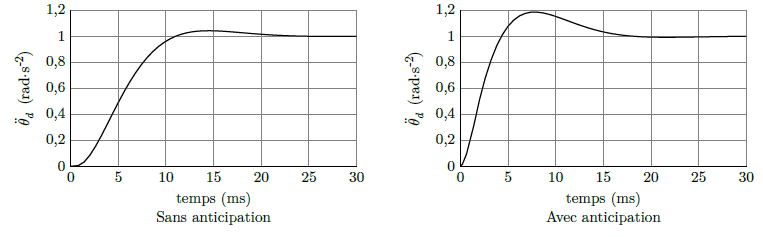
\includegraphics[width=1.0\linewidth]{image18.png}
\textit{Accélération du dosseret avec et sans anticipation \label{fig17}}
\end{center}
%\end{figure}
\fi

\subparagraph{}\textit{Conclure quant au respect du cahier des charges vis-à-vis des
  accélérations produites par le dosseret du siège dynamique de cinéma.}
\ifprof
\begin{corrige}
\end{corrige}
\else
\fi

%%\FloatBarrier

\subsection*{Exigence fonctionnelle << incliner le spectateur suivant l'axe de tangage et de roulis >>}
%
%\begin{obj}
%Valider le choix de conception permettant de transmettre l'énergie mécanique à l'assise du siège.
%\end{obj}

%\subsubsection*{Commande en simultanée des deux moteurs de l'assise du siège}

\begin{obj}

Valider le choix de conception pour la réalisation de la commande simultanée des deux moteurs de l'assise du siège.
\end{obj}

\ifprof
\else

En mode simultané (figure suivante), les consignes de vitesse de chaque
variateur sont issues d'un calculateur numérique : a, d et c sont
identiques. En revanche, le réglage du retour vitesse des cartes
variateur est effectué à l'aide d'un potentiomètre et celui-ci peut ne
pas avoir été réglé avec précision. En imposant le réglage du retour
vitesse de la motorisation 1 à 5 V pour $\SI{3000}{tr.min^{-1}}$
et celui de la motorisation 2 à \SI{5,5}{V} pour $\SI{3000}{tr. min^{-1}}$,

les calculs donnent b\textsubscript{1} = 62,8
rad.s\textsuperscript{-1}.V\textsuperscript{-1} et b\textsubscript{2} =
57,1 rad.s\textsuperscript{-1}.V\textsuperscript{-1}. Les inerties au
niveau de chaque moteur, supérieures à celle au niveau du moteur de
dosseret, peuvent fluctuer en fonction de la position du spectateur.

En tenant compte d'une variation d'inertie de 10\%, les calculs donnent
$\tau$\textsubscript{1} = 1/366 s et $\tau$\textsubscript{2} = 1/447 s. On prendra
$a =\SI{0,09}{V}$, $c =\SI{40}{rad^{-1}}$ et $d = \SI{0,016}{V.rad^{-1}.s}$.


%\begin{figure}[!htb]
\begin{center}
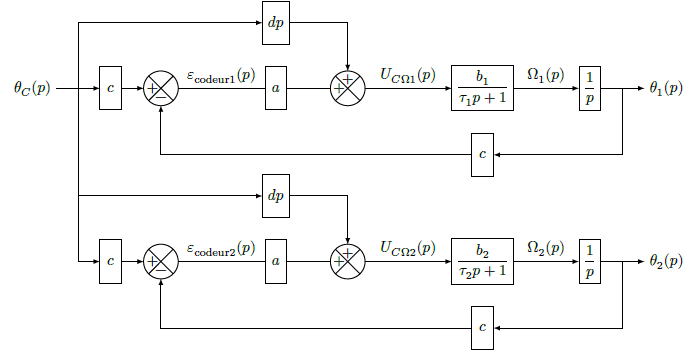
\includegraphics[width=1.0\linewidth]{image20.png}
\textit{Commande simultanée des deux moteurs \label{fig19}}
\end{center}
%\end{figure}

\fi

\subparagraph{}\textit{En réutilisant éventuellement les calculs effectués aux questions \ref{q13} et \ref{q14} et en
  tenant compte des différences de réglage de retour vitesse et des
  différences d'inertie entre les deux motorisations, exprimer la valeur
  finale de $\theta_1(t)-\theta_2(t)$ lorsque la consigne $\theta_C(t)$ est respectivement
  égale à $u(t)$, $t\cdot u(t)$ puis \(\frac{t^{2}}{2}u(t),\) $u(t)$ étant la
  fonction échelon unité.}
\ifprof
\begin{corrige}
En raisonnant graphiquement, on a $\theta_1(p)- \theta_2(p)=\varepsilon_{\text{codeur 1}}(p)- \varepsilon_{\text{codeur 2}}(p)$; donc : 
\begin{itemize}
\item $\mu_p = \mu_{p1}-\mu_{p2} = 0$;
\item $\mu_v = \mu_{v1}-\mu_{v2} = \dfrac{1-b_1d}{ab_1}-\dfrac{1-b_2d}{ab_2} $ ;
\item $\mu_a = \mu_{a1}-\mu_{a2} = \infty$.
\end{itemize}
\end{corrige}
\else
\fi

La figure \ref{fig20} représente le résultat d'une simulation de
$\theta_1(t)-\theta_2(t)$ pour une
consigne \(\theta_{C}\ \left( t \right) = \ \frac{t^{2}}{2}U(t)\)

\subparagraph{}\textit{Conclure quant à l'erreur en accélération lors de la commande
  simultanée.}
\ifprof
\begin{corrige}
\end{corrige}
\else
\fi

\ifprof
\else


%\begin{figure}[!htb]
\begin{center}
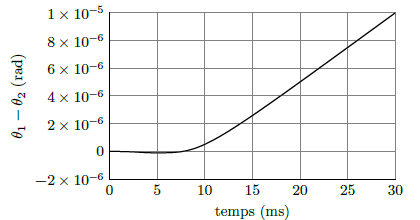
\includegraphics[width=\linewidth]{image21.png}

\textit{$\theta_1-\theta_2$ en
fonction du temps \label{fig20}}
\end{center}
%\end{figure}
\fi

\ifprof
\else
\subsection*{Éléments de correction}
\begin{enumerate}
\item $H_{\Omega}(p)=\dfrac{\dfrac{1}{K_{\Omega}}\left( 1 + T_{1}p \right)}{\dfrac{T_{1} K_{rI}J}{K_{\Omega}k_{1}K}p^2+\left(\dfrac{f K_{rI}}{K_{\Omega}k_{1}K}+1\right)T_{1}p + 1 }$.
\item  $b=\dfrac{1}{K_{\Omega}} = 20 \pi = \SI{62,8}{rad.s{-1}V^{-1}}$ et $\tau=\dfrac{K_{ri}J}{k_1KK_{\Omega}}=\SI{2,17e-3}{s}$.
\item $-\dfrac{T_{1}K_{ri}p}{ k_{1}\left( T_{1}p + 1 \right)K}\cdot \dfrac{b}{p\left(1+\tau p \right)+abc}$ et $\lim\limits_{t\to\infty} \theta(t) = 1$.
\item  ${a}=\dfrac{1}{4bc\tau\xi^2}=0,092$.
\item $\mu(p)=\dfrac{p\left( 1+\tau p\right)}{p\left( 1+\tau p\right)+abc}\theta_c(p)$, $\mu_p = 0$, $\mu_v = \dfrac{1}{abc}$ et  $\mu_a = \infty$.
\item $\mu_p=0$ et $\mu_v= \dfrac{1 -bd}{ab}$.
\item ...
\item ...
\item ...
\item ...
\end{enumerate}
\fi


\ifprof
\else
\end{multicols}
\fi

%\begin{center}
%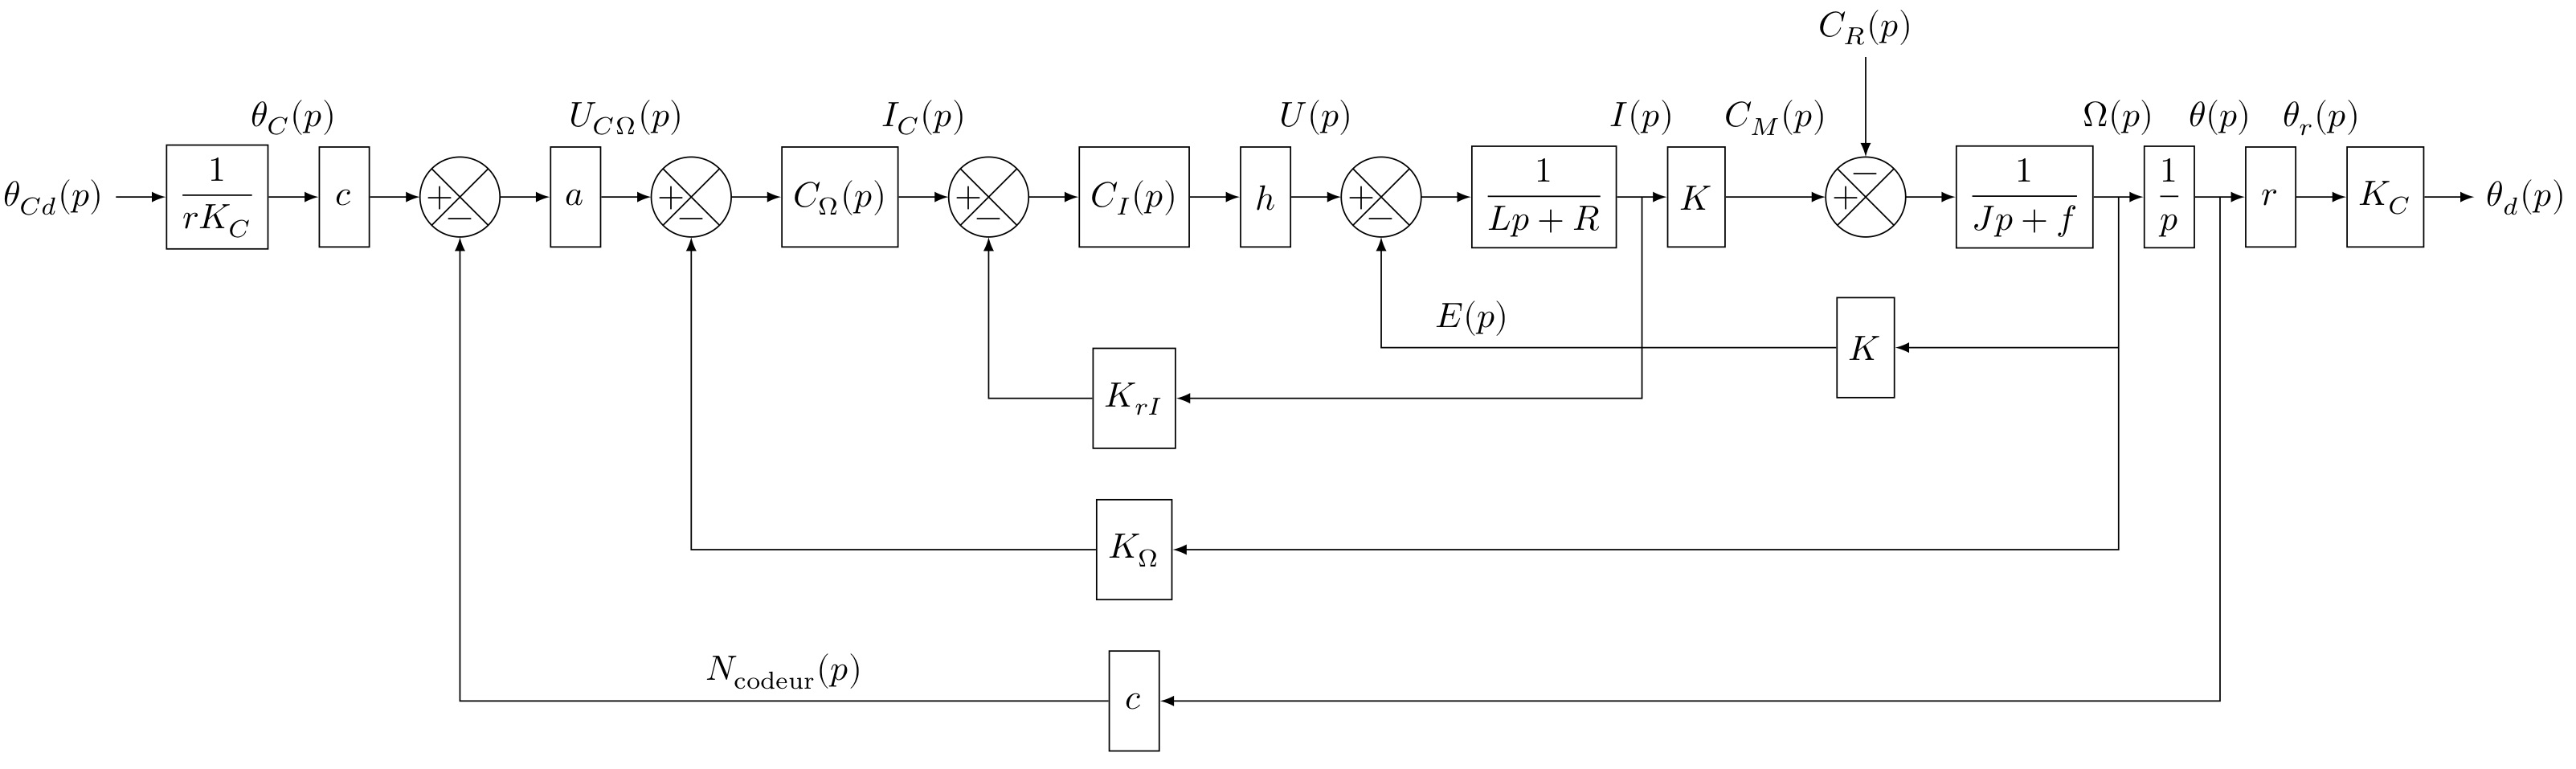
\includegraphics[width=\linewidth]{schema_bloc.jpg}
%
%\textit{Schéma-blocs de l'asservissement du dosseret \label{fig6}}
%\end{center}
%
%\end{document}
%
%\subparagraph{}\textit{}
%\ifprof
%\begin{corrige}
%\end{corrige}
%\else
%\fi
%
%\begin{center}
%\includegraphics[width=\linewidth]{}
%%\textit{}
%\end{center}
%\begin{center}
%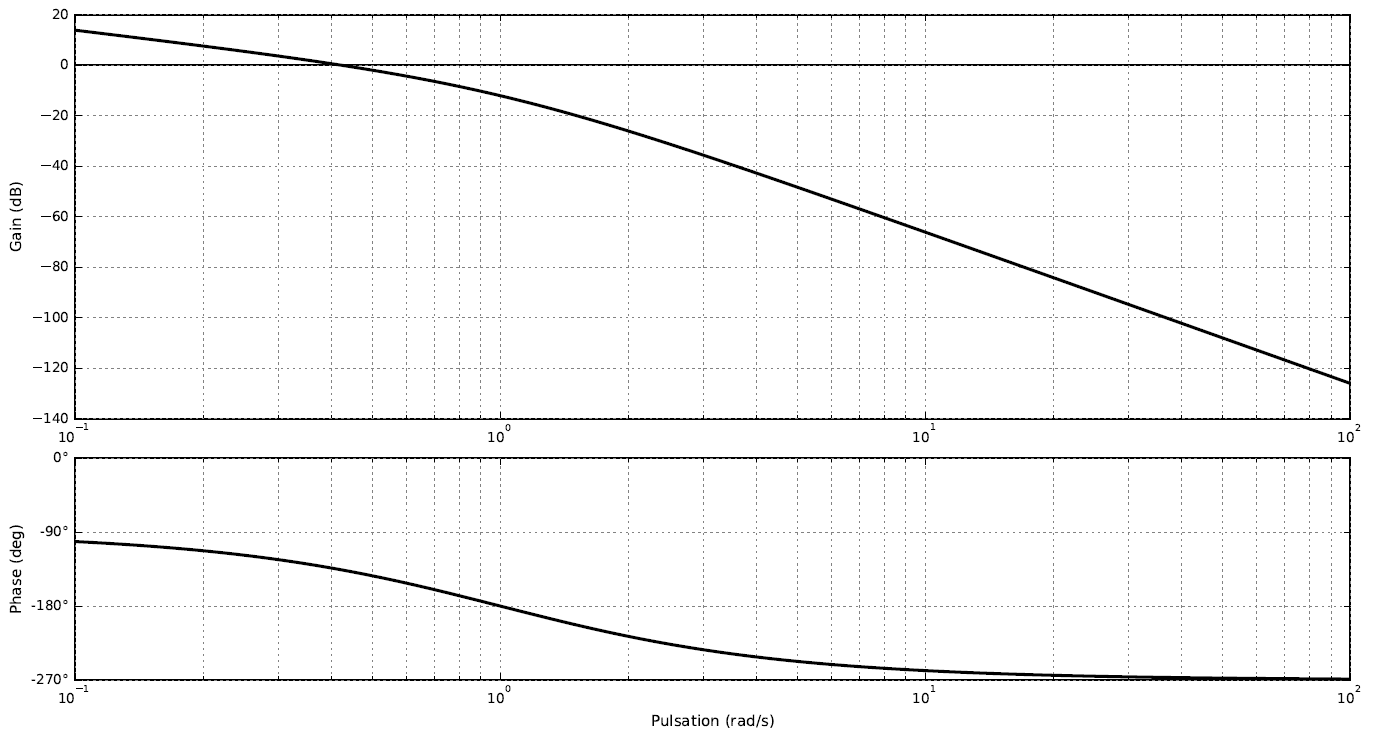
\includegraphics[width=\linewidth]{img_04}
%%\textit{}
%\end{center}
%
